\RequirePackage{snapshot}
\documentclass[twoside,a4paper,11pt]{memoir}
\usepackage{thesis}

\addbibresource{bib.bib}

% !TEX root = thesis.tex

\title{A type system for dynamic instances}
\subtitle{Version of \today}
%\subtitle{Master's Thesis}
\author{Albert ten Napel}
\authoremail{\url{a.tennapel@student.tudelft.nl}}
\birthplace{Urk, the Netherlands}
\studentid{4087798}
\coverpicture{\includegraphics[width=13cm]{./img/maze.ps}}
\colophon{\noindent
  \copyright{} \the\year{} \: Albert ten Napel. \\[1em]
  Cover picture: Random maze.
}


%\usepackage{xcolor}
\usepackage{mdframed}
%\usepackage{colorbox}
\usepackage{listings}
\usepackage{mathtools}
%\usepackage{amsmath}
%\usepackage{tabularx}
\usepackage{adjustbox}
\usepackage{amsthm}
\usepackage{capt-of}
\usepackage{minted}
\usepackage{fitch}
%\usepackage[parfill]{parskip}
\usepackage{empheq}
\usepackage{multicol}
\usepackage{mathpartir}
\usepackage{scalerel}

% infer macros
%\usepackage{hyperref}
\usepackage{pftools}
\usepackage{locallabel}

\usepackage{enumitem}
\setlist{nolistsep}

%\usepackage{cleveref}
%\crefname{section}{§}{§§}
%\Crefname{section}{§}{§§}
%\crefformat{section}{§#2#1#3}

\setminted{
	breaklines=false,
	breakanywhere=false,
	breakbytoken=false,
}

\setlength{\parindent}{0pt}

\newtheorem{lemma}{Lemma}
\newtheorem{sublemma}{Lemma}[lemma]

\newtheorem{theorem}{Theorem}

\def\allowhash{%%%%
    \bgroup\everyeof{\egroup}\catcode35=11\relax\scantokens}%

\newcommand\ident[1]{\mintinline{haskell}{#1}}
\newcommand\identp[1]{\mintinline{text}{#1}}

\newcommand{\lang}{Miro}

\undef\ulcorner
\undef\urcorner
\undef\llcorner
\undef\lrcorner
\usepackage{amssymb}
%\newcommand{\varnothing}{\emptyset}

\lstset{
	frame = single,
	basicstyle=\ttfamily\footnotesize,
	breaklines=false
}

% \title{A type system for algebraic effects and handlers with dynamic instances}
% \author{Albert ten Napel}
% \date{}

\begin{document}

\frontmatter
\thispagestyle{empty}
\maketitle
\makeformaltitlepages{% !TEX root = thesis.tex
Side-effect are ubiquitous in programming. Examples include mutable state, exceptions, nondeterminism, and user input.
Algebraic effects and handlers are an approach to programming that gives a structured way of programming with effects.
Each effect in a system with algebraic effects is defined by a set of operations.
These operations can then be called anywhere in a program.
Using a handler we can give an interpretation for the operations used.
Unfortunately we are unable to express dynamic effects such as the dynamic creation of mutable references using regular algebraic effects.
Extending algebraic effects with effect instances enabled us to express dynamic effects.
These effect instances can be dynamically created and operations called on them are distinct from the same operation called on a different instance.
Without a type system these dynamic instances may result in runtime errors, because operations may
Because of their dynamic nature it is hard to give a type system for these dynamic instances though.
In this thesis we present a new language, \lang{}, which extends algebraic effects and handlers with a restricted form of effect instances.
We introduce the notion of an \emph{effect scope} which encapsulates the creation and usage of dynamically created effect instances. We give a formal description of the syntax and semantics of \lang{}.
We also give a type system which ensures that all operation calls are handled, so that we will not have runtime errors.
Because effect instances can still escape their effect scope, in computationally irrelevant parts, we encounter difficulties in proving type safety for \lang{}. We discuss these difficulties and give possible approaches to prove type safety in the future.
}

%\pagenumbering{arabic}

% !TEX root = thesis.tex

\chapter{\label{chap:Preface}Acknowledgements}
\addcontentsline{toc}{subsection}{Acknowledgements}
I would like to thank my supervisors Robbert and Casper for their invaluable feedback and for the interesting discussions.
I give my special thanks to my girlfriend Justyna, for her neverending love, support and patience.
Finally, I would like to thank my parents for their endless love and support.

\vspace{1cm}
\begin{flushright}
\theauthor{}\\
Urk, the Netherlands\\
\today{}\\
\end{flushright}


\cleardoublepage\tableofcontents
\cleardoublepage\mainmatter{}

\iffalse
\begin{enumerate}
\item Side-effects are omnipresent
\item Give examples
\item Make programs hard to understand, test, debug, hard to compile
\item many parts are pure
\item give benefits for pure parts
\item we want presice control over pure/non-pure parts
\item want to keep track of effects
\item want to use certain effects locally and encapsulated
\end{enumerate}

\textbf{Explain side-effects generally}
- side-effects
- pure, non-pure
- pros, cons
\textbf{Desires for a language}
- factor non-pure from pure
- precise control
- track effects
- encapsulation
\textbf{Algebraic effects}
- brief explanation
- pros
- cons
\textbf{Our system}
- why
\fi

Side-effects are ubiquitous in programming.
Examples include mutable state, exceptions, nondeterminism, and user input.
Side-effects often make functions hard to understand, test and debug.
This is because that every invocation of the function with the same arguments may yield different results.
Furthermore side-effectful programs can also be difficult to optimize, since the compiler does not have much freedom in rearranging parts of the program.
\\\\
Any function that includes such effects is called impure, while functions whose only effect is computing a result are called pure.
Pure functions on the other hand do not rely on any global state and thus can be reasoned about in isolation of the rest of the program.
Every time a pure function is called with the same input, it will return the same output.
This means those functions are easier to understand, test and debug.
\\\\
There has been a lot of work on programming languages that allow more control over the pure and impure parts of a program.
Examples include Haskell\cite{haskell}, Eff\cite{eff1}, Koka\cite{koka2}, and Links\cite{links}.
These languages, in one way or another, give the programmer more control over which parts of their program are pure and which parts are impure.
By factoring out the pure parts from the impure parts, we can still gain the benefits of pure functions for many parts of our programs.
In addition it would be even better to be able to keep track of which effects exactly are used by which function.
They also allow some side-effects to be encapsulated, meaning that the use of a particular side-effect can be completely hidden such that the function still appears to be pure to the outside world.
\\\\
Type systems appear in all kinds of languages.
A type system statically enforces certain properties, different languages may have different type systems that enforce different properties.
Usually a type system is used to statically encode the expected value and return types of a function.
This ensures that a function does not receive an argument that is unable to compute with.
In the case of effect-full language a type system can do even more.
Using a type-and-effect system function can be statically annotated with the side-effects that may occur in that function.
This gives more insight to the programmer and the compiler in to what a function may do when called.
\\\\
Algebraic effects and handlers\cite{algeff} are an approach to programming with side-effects that has many of the desirable properties previously described.
Each effect is defined as a set of operations, for example nondeterminism can be represented by an operation which takes to values and chooses one.
Similarly, state can be defined as two operations, get and put, where get is meant to return the current value of the state and put is meant to change this value.
Functions are tagged by the set of effects they may use.
These operations can then be called anywhere in a function.
Handlers take a program that calls operations and for each operation call defines how to proceed.
Most side-effects that are used in programming can be defined in this system.
Algebraic effects provide a way to factor out the pure parts, the operation calls, from the impure parts, the handlers.
Furthermore functions using different algebraic effects compose just as easily as pure functions do.
There also have been multiple type-and-effect systems that can handle algebraic effects\cite{eff2}\cite{koka1}\cite{links}.
For example the following piece of code defines an effect called \textit{State} which simulates a single mutable state cell.
The function \mintinline{haskell}{postInc} increments the current value in the state cell and returns the previous value.
\begin{minted}[tabsize=2]{haskell}
effect State {
	get : () -> Int
	put : Int -> ()
}

postInc : Int!{State}
postInc =
	x <- get ();
	put (x + 1);
	return x
\end{minted}

While algebraic effects and handlers have many of the desirable properties we would like, it is unable to express multiple mutable state cells.
In the previous example it can be seen that \mintinline{haskell}{postInc} does not refer to any variables, but instead can only manipulate the mutable state using the get and put operations.
In Haskell the the so-called ``ST monad''\cite{runst} can be used to safely implement multiple mutable state cells in such a way that stateful computations can be encapsulated and that the references to the mutable objects are not leaked outside of the function. 
A feature called dynamic instances was introduced by the Eff programming language\cite{eff1}.
With dynamic instances multiple different instances of the same effect can be dynamically created.
Using this multiple state cells can be implemented.
Unfortunately there is no type-and-effect for dynamic instances, using them can results in runtime errors when instances do not have an associated handler.
\\\\
In this thesis we define a calculus based on algebraic effects and handlers which allows for the definition of side-effects such as local references, local exceptions, and the dynamic opening of channels.
Using this system we can implement a system similar to the ``ST monad'' in Haskell.
This system gives full control of which parts of a program are pure and impure.
Functions also compose easily, irrelevant of which side-effects they use.
Using a type-and-effect system we every function keeps track of which effects it may use.
We also statically ensure that side-effects are encapsulated.
We give examples of programs using these side-effects in our system and show how to implement local mutable references in this system.
We give a formal description of the syntax, typing rules and semantics of the system.

\section{Contributions}
\begin{itemize}

\item \textbf{We define a calculus based on algebraic effects and handlers which allows for the definition of local mutable state.}
We define a type-and-effect system which ensures that references do not escape their scope.
We also define a small-step operation semantics.

\item \textbf{We show how to implement state threads in this system.}
Using our sytem we implement state threads similar to a monomorphic version Haskell's ST-monad.
We show that references cannot escape their scope and that we cannot use a variable from one state thread in another state thread.

\end{itemize}

\section{Thesis structure}


\chapter{\label{chap:algintro}An introduction to algebraic effects and handlers}

Side-effects are an essential part of a programming language. Without side-effects the program would have no way to print a result to the screen, ask for user input or change global state. We consider a function pure if it does not perform any side-effects and unpure if it does. A pure function always gives the same result for the same inputs. A pure function can be much easier to reason about than an unpure one because you know that it won't do anything else but compute, it won't have any hidden inputs or outputs. Because of this property testing pure functions is also easier, we can just give dummy inputs to the functions and observe the output. As already said programs without side-effects are useless, we would not be able to actually observe the result of a function call without side-effects such as printing to the screen. So we would the benefits of pure functions but still have side-effects. We could give up and simply add some form of side-effects to our language but that would immediately make our function impure, since any function might perform side-effects. This would make us lose the benefits of pure functions.
\\\\
Algebraic effects and handlers are a structured way to introduce side-effects to a programming language.
The basic idea is that side-effects can be described by sets of operations, called the interface of the effect.
Operations from different effects can then be called in a program.
These operations will stay abstract though, they will not actually do anything.
Instead, similar to exceptions where exceptions can be thrown and caught, operations can be ``caught'' by handlers.
Different from exceptions however the handler also has access to a continuation which can be used to continue the computation at the point where the operation was called.
\\\\
In this chapter we will introduce algebraic effects and handlers through examples.
Starting with simple algebraic effects and handlers (\cref{sec:background-algeff}).
After we will continue with static instances (\cref{sec:background-staticinst}) which allows for multiple static instances of the same effect to be used in a program.
We end with dynamic instances (\cref{sec:background-dynamicinst}) which allows for the dynamic creation of effect instances. The examples are written in a statically typed functional programming language with algebraic effects and handlers with syntax reminiscent to Haskell but semantically more similar to Koka~\autocite{koka2}.

\section{Algebraic effects and handlers}
\label{sec:background-algeff}
We will start with the familiar exceptions. We define an \ident{Exc} effect interface with a single operation \ident{throw}.

\begin{minted}[tabsize=2]{haskell}
effect Exc {
	throw : String -> Void
}
\end{minted}

For each operation in an effect interface we specify a parameter type (on the left of the arrow) and a return type (on the right of the arrow).
The parameter type is the type of a value that is given when the operation is called and that the handler also has access too.
The return type is the type of a value that has to be given to the continuation in the handler, this will be shown later.
This return value is received at the point where the operation was called.
In the case of \ident{Exc} we take \ident{String} as the parameter type, this is the error message of the exception.
An exception indicates that something went wrong and that we cannot continue in the program.
This means we do not want the program to continue at the point where the exception was thrown, which is the point where the \ident{throw} operation was called.
So we do not want to be able to call the continuation with any value.
To achieve this we specify \ident{Void} as the return type of \ident{throw}.
This is a type with no values at all, which means that the programmer will never be able to conjure up a suitable value when a value of type \ident{Void} is requested. By using \ident{Void} as the return type we can ensure that the continuation cannot be called and so that the program will not continue at the point where \ident{throw} was called. To make the code more readable we assume \ident{Void} implicitly coerces to any other type.
\\\\
We can now write functions that use the \ident{Exc} effect.
For example the following function \ident{safeDiv} which will throw an error if the right argument is $0$.
We assume here that \ident{Void} is equal to any type.

\begin{minted}[tabsize=2]{haskell}
safeDiv : Int -> Int -> Int!{Exc}
safeDiv a b =
	if b == 0 then
		throw "division by zero!"
	else
		return a / b
\end{minted}

We can call this function like any other function, but no computation will actually be performed.
The effect will remain abstract, we still need to give them a semantics.

\begin{minted}[tabsize=2]{haskell}
result : Int!{Exc}
result = safeDiv 10 2
\end{minted}

In order to actually ``run'' the effect we will need to handle the operations of that effect.
For example, for \ident{Exc} we can write a handler that returns $0$ as a default value if an exception is thrown.

\begin{minted}[tabsize=2]{haskell}
result : Int
result = handle (safeDiv 10 0) {
	throw err k -> return 0
	return v -> return v
} -- results in 0
\end{minted}

For each operation we write a corresponding case in the handler, where we have access to the argument given at operation call and a continuation, which expects a value of the return type of the operation.
There is also a case for values \ident{return}, which gets as an argument the final value of a computation and has the opportunity to modify this value or to do some final computation.
In this case we simply ignore the continuation and exit the computation early with a $0$, we also return any values without modification.
\\\\
We can give multiple ways of handling the same effect.
For example we can also handle the \ident{Exc} effect by capturing the failure or success in a sum type \ident{Either}.

\begin{minted}[tabsize=2]{haskell}
data Either a b = Left a | Right b

result : Either String Int
result = handle (safeDiv 10 0) {
	throw err k -> return (Left err)
	return v -> return (Right v)
} -- results in (Left "division by zero!")
\end{minted}

Here we return early with \ident{Left err} if an error is thrown, otherwise we wrap the resulting value using the \ident{Right} constructor.
\\\\
Another effect we might be interested in is non-determinism.
To model this we define the \ident{Flip} effect interface which has a single operation \ident{flip}, which returns a boolean when called with the unit 
value.

\begin{minted}[tabsize=2]{haskell}
effect Flip {
	flip : () -> Bool
}
\end{minted}

Using the \ident{flip} operation and if-expression we can write non-deterministic computations that can be seen as computation trees where \ident{flip} branches the tree off into two subtrees.
The following program \ident{choose123} non-deterministically returns either a $1$, $2$ or $3$.

\begin{minted}[tabsize=2]{haskell}
choose123 : Bool!{Flip}
choose123 =
	b1 <- flip ();
	if b1 then
		return 1
	else
		b2 <- flip ();
		if b2 then
			return 2
		else
			return 3
\end{minted}

Here the syntax \ident{(x <- c1; c2)} sequences the computations \ident{c1} and \ident{c2} by first performing \ident{c1} and then performing \ident{c2}, where the return value of \ident{c1} can accessed in \ident{x}.
\\\\
Again \ident{choose123} does not actually perform any computation when called, because we have yet to give it a semantics.
We could always return \ident{True} when a \ident{flip} operation is called, in the case of \ident{choose123} this will result in the first branch being picked returning $1$ as the answer.

\begin{minted}[tabsize=2]{haskell}
result : Int
result = handle (choose123) {
	flip () k -> k True
	return v -> return v
} -- returns 1
\end{minted}

Another handler could try all branches returning the greatest integer of all possibilities.

\begin{minted}[tabsize=2]{haskell}
maxresult : Int
maxresult = handle (choose123) {
	flip () k ->
		vtrue <- k True;
		vfalse <- k False;
		return (max vtrue vfalse)
	return v -> return v
} -- returns 3
\end{minted}

Here we first call the continuation \ident{k} with \ident{True} and then with \ident{False}.
The we return the maximum between those results.
\\\\
We could even collect the values from all branches by returning a list.

\begin{minted}[tabsize=2]{haskell}
allvalues : List Int
allvalues = handle (choose123) {
	flip () k ->
		vtrue <- k True;
		vfalse <- k False;
		return vtrue ++ vfalse
	return v -> return [v]
} -- returns [1, 2, 3]
\end{minted}

Again we call the continuation \ident{k} twice, but we append the two results instead.
For the \ident{return} base case we simply wrap the value in a singleton list.
\\\\
Algebraic effects have the nice property that they combine easily.
For example by combining the \ident{Exc} and \ident{Flip} we can implement backtracking, where we choose the first non-failing branch from a computation. For example we can write a function which returns all even sums of the numbers $1$ to $3$ by reusing \ident{choose123}.

\begin{minted}[tabsize=2]{haskell}
evensums123 : Int!{Flip, Exc}
evensums123 =
	n1 <- choose123;
	n2 <- choose123;
	sum <- return (n1 + n2);
	if sum % 2 == 0 then
		return sum
	else
		throw "not even!"
\end{minted}

We implement backtracking in \ident{backtrack} by handling both the \ident{flip} and \ident{throw} operations. For \ident{flip} and the \ident{return} case we do the same as in \ident{allvalues}, calling the continuation \ident{k} with both \ident{True} and \ident{False} and appending the results together. For \ident{throw} we ignore the error message and continuation and exit early with the empty list, this means that branches that results in a failure will not actually return any values.

\begin{minted}[tabsize=2]{haskell}
backtrack : List Int
backtrack () = handle (handle (evensums123) {
	flip () k ->
		vtrue <- k True;
		vfalse <- k False;
		return vtrue ++ vfalse
	return v -> return [v]
}) {
	throw msg k -> return []
	return v -> return v
} -- returns [2, 4, 4, 6]
\end{minted}

We can also handle the effects independently of each other. For example we could implement a partial version of \ident{backtrack} that only handles the \ident{Flip} effect. Any operation that is not in the handler is just passed through.

\begin{minted}[tabsize=2]{haskell}
partlybacktrack : (List Int)!{Exc}
partlybacktrack = handle (evensums123) {
	flip () k ->
		vtrue <- k True;
		vfalse <- k False;
		return vtrue ++ vfalse
	return v -> return [v]
}
\end{minted}

Now we can factor out the \ident{throw} handler into its own function.

\begin{minted}[tabsize=2]{haskell}
fullbacktrack : List Int
fullbacktrack = handle (partlybacktrack) {
	throw msg k -> return []
	return v -> return v
} -- returns [2, 4, 4, 6]
\end{minted}

Algebraic effects always commute, meaning the effects can be handled in any order.
In the backtracking example the order of the handlers does not actually matter, but in general different orders could have different results.
\\\\
Lastly we introduce the \ident{State} effect, which allows us to implement local mutable state.
We restrict ourselves to a state that consists of a single integer value, but in a language with parametric polymorphism a more general state effect could be written.

\begin{minted}[tabsize=2]{haskell}
effect State {
	get : () -> Int
	put : Int -> ()
}
\end{minted}

Our state effect has two operations, \ident{get} and \ident{put}.
The \ident{get} operation allows us to retrieve a value from the state and with the \ident{put} operation we can change the value in the state.
\\\\
We can now implement the familiar ``post increment'' operation as seen in the C programming language.
This function retrieves the current value of the state, increments it by $1$ and returns the previously retrieved value.

\begin{minted}[tabsize=2]{haskell}
postInc : Int!{State}
postInc =
	x <- get ();
	put (x + 1);
	return x
\end{minted}

To implement the semantics of the \ident{State} effect we use parameter-passing similar to how the State monad is implemented in Haskell. We will abstract the implementation of the state handler in a function \ident{runState}.

\begin{minted}[tabsize=2]{haskell}
runState : Int!{State} -> (Int -> (Int, Int))
runState comp = handle (comp) {
	get () k -> return (\s -> (f <- k s; return f s))
	put v k -> return (\s -> (f <- k (); return f v))
	return v -> return (\s -> return (s, v))
}
\end{minted}

\ident{runState} takes a computation that returns an integer and may use the \ident{State} effect, and returns a function that takes the initial value of the state and returns a tuple of the final state and the return value of the computation.
Let us take a look at the \ident{return} case first, here we return a function that takes a state value and returns a tuple of this state and the return value.
For the \ident{get} case we return a function that takes a state value and runs the continuation \ident{k} with this value, giving access to the state at the point where the \ident{get} operation was called. From this continuation we get back another function, which we call with the current state, continuing the computation without changing the state.
The \ident{put} case is similar to the \ident{get} but we call the continuation with the unit value and we continue the computation by calling \ident{f} with the value giving with the \ident{put} operation call.
\\\\
Using state now is as simple as calling \ident{runState}.

\begin{minted}[tabsize=2]{haskell}
stateResult : (Int, Int)
stateResult =
	f <- runState postInc; -- returns a function taking the initial state
	f 42 -- post-increments 42 returning (43, 42)
\end{minted}

Using the state effect we can implement imperative algorithms such as summing a range of numbers.
We first implement a recursive function \ident{sumRangeRec} which uses \ident{State} to keep a running sum.
After we define \ident{sumRange} which calls \ident{sumRangeRec} and runs the \ident{State} effect with $0$ as the initial value.

\begin{minted}[tabsize=2]{haskell}
sumRangeRec : Int -> Int -> Int!{State}
sumRangeRec a b =
	if a > b then
		(_, result) <- get ();
		return result
	else
		x <- get ();
		put (x + a);
		sumRangeRec (a + 1) b
		
sumRange : Int -> Int -> Int
sumRange a b =
	f <- runState (sumRangeRec a b);
	f 0 -- initial sum value is 0
\end{minted}

\section{Static instances}
\label{sec:background-staticinst}

Static instances extend algebraic effects by allowing multiple instances of the same effect to co-exist.
These instances be handled independently of each other.
Operations in such a system are always called on a specific instance and handlers also have to note instance they are handling.
We will write operation calls as \allowhash{\ident{inst#op(v)}} where \ident{inst} is the instance.
Handlers are modified to take an instance parameter as follows \allowhash{\ident{handle#inst(comp) { ... }}}.
\\\\
As an example let us take another look at the \ident{safeDiv} function.

\begin{minted}[tabsize=2]{haskell}
safeDiv : Int -> Int -> Int!{Exc}
safeDiv a b =
	if b == 0 then
		throw "division by zero!"
	else
		return a / b
\end{minted}

We can rewrite this to use static instances by declaring an instance of \ident{Exc} called \ident{divByZero} and calling the \ident{throw} operation on this instance.
Note that in the we now state the instance used instead of the effect, since multiple instances of the same effect could be used and we would like to know which instances exactly.

\begin{minted}[tabsize=2]{haskell}
instance Exc divByZero

safeDiv : Int -> Int -> Int!{divByZero}
safeDiv a b =
	if b == 0 then
		divByZero#throw "division by zero!"
	else
		return a / b
\end{minted}

Imagine we wanted to also throw an exception in the case that the divisor was negative.
Using instances we can easily declare another \ident{Exc} instance, let us call it \ident{negativeDivisor}, and use it in our function.
We also have to modify the type to mention the use of \ident{negativeDivisor}.

\begin{minted}[tabsize=2]{haskell}
instance Exc divByZero
instance Exc negativeDivisor

safeDivPositive : Int -> Int -> Int!{divByZero, negativeDivisor}
safeDivPositive a b =
	if b == 0 then
		divByZero#throw "division by zero!"
	else if b < 0 then
		negativeDivisor#throw "negative divisor!"
	else
		return a / b
\end{minted}

We can now see from the type what kind of exceptions are used in the function.
We can also handle the exceptions independently.
For example we could handle \ident{divByZero} by defaulting to \ident{0}, but leave \ident{negativeDivisor} unhandled.

\begin{minted}[tabsize=2]{haskell}
defaultTo0 : Int!{divByZero, negativeDivisor} -> Int!{negativeDivisor}
defaultTo0 c =
	handle#divByZero (c) {
		throw msg -> return 0
		return v -> return v
	}
\end{minted}

\section{Dynamic instances}
\label{sec:background-dynamicinst}

Having to predeclare every instance we are going to use is very inconvenient, especially when we have effects such as reference cells or communication channels. The global namespace would be littered with all references and channels the program would ever use. Furthermore we do not always know how many references we need. Take for example a function which creates a list of reference cells giving a length $l$. We do not know statically what the length of the list will be and so we do not know ahead how many instances we have to declare.
Furthermore because all the instances would be predeclared some information about the implementation of a function would be leaked to the global namespace. This means it is impossible to fully encapsulate the use of an effect when using static instances.
\\\\
Dynamic instances improve on static instances by allowing instances to be created dynamically.
Instances become first-class values, they can be assigned to variables and passed to functions just like any other value.
We use \ident{new E} to create a new instance of the \ident{E} effect.
The actual implementation of the function can stay exactly the same, as can the handler \ident{defaultTo0}.
We can translate the previous example to use dynamic instances by defining the \ident{divByZero} and \ident{negativeDivisor} as top-level variables and assigning newly created instances to them. We omit type annotation, since there does not exist any type system that can type all usages of dynamic instances.

\begin{minted}[tabsize=2]{haskell}
divByZero = new Exc
negativeDivisor = new Exc

safeDivPositive a b =
	if b == 0 then
		divByZero#throw "division by zero!"
	else if b < 0 then
		negativeDivisor#throw "negative divisor!"
	else
		return a / b
		
defaultTo0 c =
	handle#divByZero (c) {
		throw msg -> return 0
		return v -> return v
	}
\end{minted}

Using locally created instances we can emulate variables as they appear in imperative languages more easily.
We can implement the factorial function in an imperative style using a locally created \ident{State} instance.
The \ident{factorial} function computes the factorial of the paramter \ident{n} by creating a new \ident{State} instance named \ident{ref} and calling the helper function \ident{factorialLoop} with \ident{ref} and \ident{n}.
The base case of \ident{factorialLoop} retrieves the current value from \ident{ref} and returns it.
In the recursive case of \ident{factorialLoop} the value in \ident{ref} is modified by multiplying it by \ident{n} and then we continue by recursing with \ident{n - 1}.
The call to \ident{factorialLoop} in \ident{factorial} is wrapped in the \ident{State} handler explained earlier, chosing \ident{1} as the initial value of \ident{ref}.
\ident{factorial} thus computes the factorial of a number by using a locally created instance, but the use of this instance or the \ident{State} effect in general never escapes the function, it is completely encapsulated.

\pagebreak
\begin{minted}[tabsize=2]{haskell}
factorialLoop ref n =
	if n == 0 then
		ref#get ()
	else
		x <- ref#get();
		ref#put (x * n);
		factorialLoop ref (n - 1) 

factorial n =
	ref <- new State;
	statefn <- handle#ref (factorialLoop ref n) {
		get () k -> return (\s -> (f <- k s; return f s))
		put v k -> return (\s -> (f <- k (); return f v))
		return v -> return (\s -> return v)
	};
	statefn 1 -- use 1 as the initial value of ref
\end{minted}

Next we will implement references more generally similar to the ones available in Standard ML~\autocite{standardml}, in our case specialized to \ident{Int}.
In the previous example we see a pattern of creating a \ident{State} instance and then calling some function with it wrapped with a handler.
This is the pattern we want to use when implementing references.
To implement this pattern more generally this we first introduce a new effect named \ident{Heap}.
\ident{Heap} has one operation called \ident{ref} which takes an initial value \ident{Int} and returns a \ident{State} instance.
\ident{Heap} can be seen as a collection of references.
We then define a handler \ident{runRefs} which takes a \ident{Heap} instance and a computation, and creates \ident{State} instances for every use of \ident{ref}. After we call the continuation with the newly created instance and wrap this call in the usual \ident{State} handler, giving the argument of \ident{ref} as the initial value.

\begin{minted}[tabsize=2]{haskell}
effect Heap {
	ref : Int -> Inst State
}

runRefs inst c =
	handle#inst (c) {
		ref v k ->
			r <- new State;
			statefn <- handle#r (k r) {
				get () k -> return (\s -> (f <- k s; return f s))
				put v k -> return (\s -> (f <- k (); return f v))
				return v -> return (\s -> return v)
			};
			statefn v 
		return v -> return v
	}
\end{minted}

By calling \ident{runRefs} at the top-level we will have the same semantics for references as Standard ML.
In the following example we create two references and swap their values using a \ident{swap} function.
First \ident{main} creates a new \ident{Heap} instance \ident{heap} and then calls \ident{runRefs} with this instance.
The computation given to \ident{runRefs} is the function \ident{program} called with \ident{heap}.

\pagebreak
\begin{minted}[tabsize=2]{haskell}
swap r1 r2 =
	x <- r1#get ();
	y <- r2#get ();
	r1#put(y);
	r2#put(x)
	
program heap =
	r1 <- heap#ref 1;
	r2 <- heap#ref 2;
	swap r1 r2;
	x <- r1#get ();
	y <- r2#get ();
	return (x, y)
	
main =
	heap <- new Heap;
	runRefs heap (program heap) -- returns (2, 1)
\end{minted}

In the Haskell programming language the ST monad~\autocite{runst} can be used to implement algorithms that internally use mutable state.
The type system, using the \ident{runST} function, will make sure that the mutable state does not leak outside of the function.
For example the following function \ident{fibST} implements the Fibonacci function in constant space by creating two mutable references.

\begin{minted}[tabsize=2]{haskell}
fibST :: Integer -> Integer
fibST n = 
    if n < 2 then
      n
    else runST $ do
        x <- newSTRef 0
        y <- newSTRef 1
        fibST' n x y

    where fibST' 0 x _ = readSTRef x
          fibST' n x y = do
              x' <- readSTRef x
              y' <- readSTRef y
              writeSTRef x y'
              writeSTRef y $! x' + y'
              fibST' (n - 1) x y
\end{minted}

Using dynamic instances we can implement the same algorithm, named \ident{fib} below.
Our \ident{fib} takes a parameter \ident{n} and returns the \ident{n}th Fibonacci number.
First we check if \ident{n} is smaller than 2, in which case we can return \ident{n} as the result, since $n$th Fibonacci number is $n$, if $n < 2$.
Else we create a new \ident{Heap} instance named \ident{heap} and use the \ident{runRefs} function defined earlier to run a computation on this heap.
We create two \ident{State} instances on \ident{heap}, \ident{x} and \ident{y} initialized with \ident{0} and \ident{1} respectively and call the auxillary function \ident{fibRec} with \ident{n} and the two instances \ident{x} and \ident{y}.
\ident{fibRec} implements the actual algorithm.
It works by (recursively) looping on \ident{n}, subtracting by \ident{1} each recursive call.
\ident{x} and \ident{y} store the current and next Fibonacci respectively and each loop they are moved one Fibonacci number to the right.
When \ident{n} is \ident{0} we know \ident{x} contains the \ident{n}th (for the initial value of \ident{n}) Fibonacci number and we can just get the current value from \ident{x} and return it.
Even though this algorithm uses the \ident{Heap} and \ident{State} effects, their uses are completely encapsulated by the \ident{fib} function.
The \ident{fib} function does not leak the fact that it's using those effects to implement the algorithm.

\begin{minted}[tabsize=2]{haskell}
fib n =
  if n < 2 then
    n
  else
    heap <- new Heap;
    runRefs heap (
      x <- heap#ref 0;
      y <- heap#ref 1;
      fibRec n x y
    )

fibRec n x y =
  if n == 0 then
    x#get ()
  else
    x' <- x#get ();
    y' <- y#get ();
    x#put(y');
    y#put(x' + y');
    fibRec (n - 1) x y
\end{minted}

Dynamic instances have one big problem though: they are too dynamic. Similar to how in general it is undecidable to know whether a reference has escaped its scope, it is also not possible to know whether an instance has a handler associated with it. This makes it hard to think of a type system for dynamic instances which ensures that there are no unhandled operations. Earlier versions of the Eff programming language~\autocite{eff1} had dynamic instances but its type system underapproximated the uses of dynamic instances which meant you could still get a runtime error if any operation calls were left unhandled.


\iffalse
\fi

In this chapter we will give an introduction to programming with X. We will start with defining mutable references and mutable vectors. After we will show how to implement a list shuffling algorithm that internally uses mutation and we will finish with an example of locally scoped effects.
\\\\
We will use a language reminiscent of Haskell with algebraic data types and pattern matching.
Type constructors are uppercase while type variables are lowercase.
We will always explicitly show \ident{forall} for universally quantified scope variables.

\section{Mutable references}
To start off we will define a \ident{State} effect specialized to \ident{Int}s.
\begin{minted}[tabsize=2]{haskell}
-- the State effect
effect State {
	get : () -> Int
	put : Int -> ()
}
\end{minted}

This definition is exactly the same as the \ident{State} effect definition in Chapter~2.1, in the basic algebraic effects system.
With the \ident{effect} keyword we declare a new effect called \ident{State} with two operations: \ident{get} and \ident{put}.
For each operation we give parameter and return types. For \ident{get} we give the unit type \ident{()} as the parameter type, \ident{()} is the unit type, the type with exactly one value: the unit value, also written as \ident{()}. A parameter type of \ident{()} means that \ident{get} does not expect a meaningful argument. As the return type we give \ident{Int}, meaning that calling the \ident{get} operation will return a integer value. For the \ident{put} operation it is the other way around, as the parameter type we have \ident{Int}, meaning that \ident{put} requires an integer value when called, and the return type is \ident{()}, calling \ident{put} will give back the unit value. Having \ident{()} as the return type of an operation means that the operation does not return any meaningful value but calling the operation is only useful for its effect.
\\\\
Operations are called on an \emph{effect instance}.
As an example consider the following post-increment function:
\begin{minted}[tabsize=2]{haskell}
postInc : forall s. Inst s State -> Int!{s}
postInc inst =
	x <- inst#get ();
	inst#put (x + 1);
	return x
\end{minted}

This function takes an instance of the \ident{State} effect, called \ident{inst}, of type \ident{Inst s State}.
The meaning of the scope variable \ident{s} will be explained later, but for now you can see it as a heap where the instance ``lives''.
Operation calls can be done on an instance using the syntax \ident{instance#operation(argument)}.
We write \ident{instance#operation()} to mean \ident{instance#operation( () )}, when the unit value \ident{()} is given as the argument.
In the case of \ident{postInc} we first retrieve the current value from the instance by calling the \ident{get} operation on \ident{inst}.
This value is named \ident{x}.
After we increment the value of the instance by calling the \ident{put} operation with \ident{(x + 1)}.
\\\\
In order to use an effect we first have to create an instance of it.
We can do this using the \ident{new} keyword, for example:
\begin{minted}[tabsize=2]{haskell}
new State@s {
	get v k -> k 0
	put v k -> k ()
	return xr -> return xr
	finally xf -> return xf
} as inst in e
\end{minted}
Here we create a new instance of the \ident{State} effect at scope \ident{s} (the meaning of which we will explain later), the newly-created instance is available in the expressions \ident{e}, as the variable \ident{inst}.
When creating an instance we have to give an \emph{handler}, the handler specifies what should happen when the operations are called.
The handler is defined within curly braces and consists of a case for each operation of the effect, plus a \ident{return} case and a \ident{finally} case.
\\\\
In each operation case, \ident{get} and \ident{put} in the above example, we have access to two arguments.
The first variable, \ident{v} above, refers to the argument given when the operation was called.
The second variable, \ident{k} above, refers to the continuation of the operation call, this is the rest of the computation, after the operation call.
By calling \ident{k} with a value we can continue the computation at the point where the operation was called, at that point the program receives the value we give to the continuation \ident{k}.
In the example above we continue with \ident{0} every time \ident{get} on the instance \ident{inst} is called, and we continue with \ident{()} (without performing any other effects) whenever \ident{put} is called.
\\\\
The \ident{return} case gets called at the end of the computation \ident{e}.
The variable \ident{xf} contains the final value of the computation, which can be transformed in the case branch.
It is not required for the computation returned from the case to have the same type as \ident{xr}, and other operations are also allowed to be called.
Finally the \ident{finally} case is wrapped around the whole computation \ident{e} after the \ident{return} computation has been performed.
The variable \ident{xf} contains the transformed value returned from the \ident{return} case.
This case may not seem that useful, but we will see it is necessary in order to define mutable references.
\\\\
Explain scopes here.
\\\\
Example of references

\begin{minted}[tabsize=2]{haskell}
-- create a fresh reference initialized with the integer value v
newRef : forall s. t -> (Inst s State)!{State@s}
newRef [s] v =
	new State@s {
		get () k -> \s -> k s s
		put s' k -> \s -> k () s'
		return x -> \s -> return x
		finally f -> f v
	} as x in return x
\end{minted}
explanation.
\\\\
Example of using references

\section{Mutable vectors}
\begin{minted}[tabsize=2]{haskell}
-- (linked) list of integer values
data List = Nil | Cons Int List

-- a mutable vector modeled by
-- a list of references in scope s
type Vector s = List (Inst s State)

-- get the length of a list
length : List -> Int
length Nil = 0
length (Cons _ t) = 1 + (length t)

-- transform a list to a vector by replacing each value in the list
-- by a reference initialized with that value
toVector : forall s. List -> (Vector s)!{State@s}
toVector [s] Nil = Nil
toVector [s] (Cons h t) =
	h' <- newRef [s] h;
	t' <- toVector [s] t;
	return (Cons h' t')

-- transform a vector back to a list by getting the
-- current values from the references in the vector
toList : forall s. Vector s -> List!{State@s}
toList [s] Nil = Nil
toList [s] (Cons h t) =
	h' <- h#get();
	t' <- toList [s] t;
	return (Const h' t')

-- get the value at the index given as the first argument
-- assumes the index is within range of the vector
vget : forall s. Int -> Vector s -> Int!{State@s}
vget [s] 0 (Cons h _) = h#get()
vget [s] n (Cons _ t) = vget [s] (n - 1) t

-- set the value at the index given as the first argument
-- to the value given as the second argument
-- assumes the index is within range of the vector
vset : forall s. Int -> Int -> Vector s -> ()!{State@s}
vset [s] 0 v (Cons h _) = h#put(v)
vset [s] n v (Cons _ t) = vset [s] (n - 1) v t
\end{minted}

\section{List shuffle}
\begin{minted}[tabsize=2]{haskell}
-- random number generation effect
-- the operation `rand` gives back a random integer
-- between 0..n, where n is the argument given (exclusive)
effect Rng {
	rand : Int -> Int
}

-- shuffles a list given an instance of Rng
shuffle : forall s'. Inst s' Rng -> List -> List!{Rng@s'}
shuffle [s'] rng lst =
	handle(s ->
		let vec = toVector [s] lst;
		shuffleVector [s] [s'] rng 100 vec;
		return (toList vec))

-- shuffles a vector given an instance of Rng
-- by swapping two random elements of the vector
-- the second argument to shuffleVector is the amount of times
-- to swap elements
shuffleVector : forall s s'. Inst s' Rng -> Int -> Vector s -> ()!{State@s, Rng@s'}
shuffleVector [s] [s'] _ 0 vec = vec
shuffleVector [s] [s'] rng n vec =
	let len = length vec;
	i <- rng#rand(len);
	j <- rng#rand(len);
	a <- vget [s] i vec;
	b <- vget [s] j vec;
	vset [s] i b vec;
	vset [s] j a vec;
	shuffleVector [s] [s'] rng (n - 1) vec
\end{minted}

\section{Local effects}
\begin{minted}[tabsize=2]{haskell}
-- folding with early exit
effect Done t {
	done : t -> ()
}

-- foldr creates a new instance of Done
-- and passes this to the reducer function
-- if done is called on the instance
-- then foldr stops and returns the value given
-- note: nested uses of foldr do not interfere because
-- new instances are created with each call
foldr : (forall s. Inst s (Done r) -> Int -> r -> r!{(Done r)@s}) ->
	r -> List -> r
foldr fn initial list =
	handle(s ->
		new Done@s {
			done v k -> return v
			return x -> return x
		} as inst in
		foldrRec [s] (fn [s] inst) initial list)

-- recursive foldr implementation
foldrRec : forall s. (Int -> r -> r!{(Done r)@s}) ->
	r -> List -> r!{(Done r)@s}
foldRec fn initial Nil = initial
foldRec fn initial (Cons h t) = fn h (foldRec fn initial t)

-- does the list have any element satifying the predicate function
-- returns early if the predicate function returns True
contains : (Int -> Bool) -> List -> Bool
contains fn list =
	let result = foldr (\inst h _ ->
		if fn h then
			inst#done(True)
		else
			False
	) False list
\end{minted}

\section{Type inference for STLC}
\begin{minted}[tabsize=2]{haskell}
data Maybe t = Nothing | Just t

effect Fail {
	fail : () -> Void
}

effect MetaVar {
	assign : Ty s -> ()
	get : () -> Maybe (Ty s)
}

data Term = Var String | Abs String Term | App Term Term
type MVar s = Inst s MetaVar
data Ty s = TVar (MVar s) | TFun Ty Ty

freshMVar : forall s. (MVar s)!{MetaVar@s}
freshMVar [s] () =
	new MetaVar@s {
		assign t k -> 	return \mty -> k () (Just t)
		get () k -> 	return \mty -> k mty mty
		return f -> f Nothing
	} as mv in return mv

pruneMVar : forall s. MVar s -> (Ty s)!{MetaVar@s}
pruneMVar [s] mv =
	mty <- mv#get();
	case mty of
		Nothing -> TVar mv
		Just t ->
			let t' = prune [s] t;
			mv#assign(t');
			return t'

prune : forall s. Ty s -> (Ty s)!{MetaVar@s}
prune [s] (TVar mv) = pruneMVar [s] mv
prune [s] (TFun a b) = TFun (prune [s] a) (prune [s] b)

unify : forall s. Inst s Fail -> Ty s -> Ty s -> ()!{MetaVar@s, Fail@s}
unify [s] fail (TVar mv) t = assignMVar [s] fail x t
unify [s] fail t (Var mv) = assignMVar [s] fail x t
unify [s] fail (TFun l1 r1) (TFun l2 r2) =
	unify [s] fail l1 l2;
	unify [s] fail r1 r2
unify [s] fail _ _ = fail#fail()

assignMVar : forall s. Inst s Fail -> MVar s -> Ty s -> ()!{MetaVar@s}
assignMVar [s] fail x (TVar y) | x == y = return ()
assignMVar [s] fail x t =
	let ty = pruneMVar [s] x;
	case ty of
		TVar mv -> mv#assign(t)
		_ -> unify [s] fail ty t

data Env s = ENil | ECons String (Ty s) (Env s)

extend : forall s. String -> Ty s -> Env s -> Env s
extend [s] x t e = ECons x t e

lookup : forall s. String -> Env s -> Maybe (Ty s)
lookup [s] x ENil = Nothing
lookup [s] x (ECons y ty _) | x == y = Just ty
lookup [s] x (ECons _ _ rest) = lookup [s] x rest

infer : forall s. Inst s Fail -> Env -> Term -> (Ty s)!{MetaVar@s, Fail@s}
infer [s] fail env (Var x) =
	case (lookup x env) of
		Just ty -> return ty
		Nothing -> fail#fail()
infer [s] fail env (Abs x b) =
	mv <- freshMVar [s];
	let env' = extend x (TVar mv) env;
	ty <- infer [s] fail env' b;
	return (TFun (TVar mv) ty)
infer [s] fail env (App a b) =
	ta <- infer [s] fail env a;
	tb <- infer [s] fail env b;
	mv <- freshMVar [s];
	unify [s] fail ta (TFun tb (TVar mv));
	return (TVar mv)

data FinalTy = FTVar Int | FTFun FinalTy FinalTy

finalizeTy : forall s. Inst s State -> Ty s -> FinalTy!{MetaVar@s, State@s}
finalizeTy [s] ref (TVar mv) =
	ty <- mv#get();
	case ty of
		Just t -> finalizeTy [s] ref t
		Nothing ->
			i <- ref#get();
			ref#put(i + 1);
			mv#assign(FTVar i);
			return (FTVar i)
finalizeTy [s] ref (TFun a b) =
	a' <- finalizeTy [s] ref a;
	b' <- finalizeTy [s] ref b;
	return (FTFun a' b')

inferTop : Env -> Term -> Maybe FinalTy
inferTop [s] env term =
	handle(s ->
		new Fail@s {
			fail () k -> return Nothing
			return x -> return x
		} as fail in
		ty <- infer [s] fail env term;
		pruned <- prune ty;
		fty <- finalizeTy pruned;
		return (Just fty))
\end{minted}


{
\newcommand\synchange[1]{\colorbox{lightgray}{$#1$}}

\newcommand\eff[0]{\epsilon}
\newcommand\Eff[0]{E}
\newcommand\Op[1]{O^{#1}}

% types
\newcommand\ty[0]{\tau}
\newcommand\tunit[0]{()}
\newcommand\tarr[2]{#1 \rightarrow #2}
\newcommand\thandler[2]{#1 \Rightarrow #2}
\newcommand\tforall[3]{\forall(#1:#2) . #3}
\newcommand\tinst[1]{\mathsf{inst}(#1)}

% computation type
\newcommand\cty[0]{\underline{\ty}}
\newcommand\aty[2]{#1 \; ! \; #2}
\newcommand\texists[3]{\exists(#1:#2) . #3}
\newcommand\texistss[2]{\exists \overrightarrow{#1} . #2}
% values
\newcommand\val[0]{\nu}
\newcommand\vunit[0]{()}
\newcommand\vinst[0]{\iota}
\newcommand\vabst[3]{\Lambda(#1:#2) . #3}
\newcommand\vabs[2]{\lambda #1 . #2}
\newcommand\vappt[2]{#1 \; [ #2 ]}

% computations
\newcommand\comp[0]{c}
\newcommand\creturn[1]{\mathsf{return} \; #1}
\newcommand\capp[2]{#1 \; #2}
\newcommand\cdo[3]{#1 \leftarrow #2 ; #3}
\newcommand\cop[2]{#1(#2)}
\newcommand\copi[3]{#1 \# #2(#3)}
\newcommand\chandle[2]{\mathsf{handle} (#1) \{ #2 \}}
\newcommand\chandlei[3]{\mathsf{handle}^{#1} (#2) \{ #3 \}}
\newcommand\cnew[1]{\mathsf{new} \; #1}
\newcommand\cunpack[4]{(#1, #2) \leftarrow #3 ; #4}

%handlers
\newcommand\hop[5]{#1 \; #2 \; #3 \rightarrow #4 ; \; #5}
\newcommand\hreturn[2]{\mathsf{return}\; #1 \rightarrow #2}
\newcommand\hopc[4]{#1 \; #2 \; #3 \rightarrow #4}

\chapter{\label{chap:algtheory}Semantics and types of algebraic effects and handlers}

In this chapter we will give a theoretical basics for algebraic effects and handlers as introduced in \cref{chap:algintro}.
We do this in order to ease the reader in to the theoretical calculus for \lang{} (given in \cref{chap:langtheory}) which is based on the calculus for algebraic effects given in this chapter.
We will start with the simply-typed lambda calculus (\cref{sec:theory-stlc}) and then add algebraic effects (\cref{sec:theory-algeff}) and static instances (\cref{sec:theory-staticinst}) to it.

\section{Simply-typed lambda calculus} \label{sec:theory-stlc}

As our base language we will take the fine-grained call-by-value simply-typed lambda calculus (FG-STLC) \autocite{fg-stlc}.
This system is a version of the simply-typed lambda calculus with a syntactic distinction between values and computations.
Because of this distinction there is exactly one evaluation order: call-by-value.
In a system with side effects the evaluation order is very important since a different order could have a different result.
Having the evaluation order be apparent from the syntax is thus a good choice for a system with algebraic effects.
Another way to look at FG-STLC is to see it as a syntax for the lambda calculus that constrains the program to always be in A-normal form \autocite{anormalform}.

%\subsection{Syntax}

\begin{figure}
\caption{Syntax of the fine-grained lambda calculus}
\centering
\fbox{
\begin{minipage}{6 cm}
\begin{align*}
& \val \Coloneqq x, y, z, k \;|\; \vabs{x}{\comp} \;|\; \vunit \\
& \comp \Coloneqq \creturn{\val} \;|\; \capp{\val}{\val} \;|\; \cdo{x}{\comp}{\comp}
\end{align*}
\label{fig:syntax-stlc}
\end{minipage}
}
\end{figure}

The terms are shown in \cref{fig:syntax-stlc}.
The terms are split in to values and computations.
Values are pieces of data that have no effects, while computations are terms that may have effects.

\paragraph{Values} We have $x$, $y$, $z$, $k$ ranging over variables, where we will use $k$ for variables that denote continuations later on.
Lambda abstractions are denoted as $\vabs{x}{\comp}$, note that the body $\comp$ of the abstraction is restricted to be a computation as opposed to the ordinary lambda calculus where the body can be any expression.
To keep things simple we take unit $\vunit$ as our only base value. Adding more base values will not complicate the theory.
Using the unit value we can also delay computations by wrapping them in an abstraction that takes a unit value.
\\\\
\paragraph{Computations} For any value $\val$ we have $\creturn{\val}$ for the computation that simply returns a value without performing any effects. We have function application $(\capp{\val}{\val})$, where both the function and argument have to be values. Sequencing computations is done with $(\cdo{x}{\comp}{\comp})$. Normally in the lambda calculus the function and the argument in an application could be any term and so a choice would have to be made in what order these have to be evaluated or whether to evaluate the argument at all before substitution. In the fine-grained calculus both the function and argument in $(\capp{\val}{\val})$ are values so there is no choice of evaluation order. The order is made explicit by the sequencing syntax $(\cdo{x}{\comp}{\comp})$.

%\subsection{Semantics}

\begin{figure}
\caption{Semantics of the fine-grained lambda calculus}
\centering
\fbox{
\begin{minipage}{12 cm}
\begin{mathpar}
\inferH{S-App}{
}{
	\capp{(\vabs{x}{\comp})}{\val} \rightsquigarrow \comp[x := \val]
}
\and
\inferH{S-SeqReturn}{
}{
	(\cdo{x}{\creturn{\val}}{\comp}) \rightsquigarrow \comp[x := \val]
}
\and
\inferH{S-Seq}{
	\comp_1 \rightsquigarrow \comp_1'
}{
	(\cdo{x}{\comp_1}{\comp_2}) \rightsquigarrow (\cdo{x}{\comp_1'}{\comp_2})
}
\end{mathpar}
\label{fig:semantics-stlc}
\end{minipage}
}
\end{figure}

\paragraph{Semantics}
The small-step operational semantics is shown in \cref{fig:semantics-stlc}.
The relation $\rightsquigarrow$ is defined on computations, where the $\comp \rightsquigarrow \comp'$ means $\comp$ reduces to $\comp'$ in one step.
These rules are a fine-grained approach to the standard reduction rules of the simply-typed lambda calculus.
In {\footnotesize\textsc{S-App}} we apply a lambda abstraction to a value argument, by substituting the value for the variable $x$ in the body of the abstraction.
In {\footnotesize\textsc{S-SeqReturn}} we sequence a computation that just returns a value in another computation by substituting the value for the variable $x$ in the computation.
Lastly, in {\footnotesize\textsc{S-Seq}} we can reduce a sequence of two computations, $\comp_1$ and $\comp_2$ by reducing the first, $\comp_1$.
\\\\
We define $\rightsquigarrow^*$ as the transitive-reflexive closure of $\rightsquigarrow$.
Meaning that $\comp$ in $\comp \rightsquigarrow^* \comp'$ can reach $\comp'$ in zero or more steps, while $\comp$ in $\comp \rightsquigarrow \comp'$ reaches $\comp'$ in exactly on step.

%\subsection{Type system}

\begin{figure}
\caption{Types of the fine-grained simply-typed lambda calculus}
\centering
\fbox{
\begin{minipage}{4 cm}
\begin{align*}
& \ty \Coloneqq \tunit \;|\; \tarr{\ty}{\cty} \\
& \cty \Coloneqq \ty
\end{align*}
\label{fig:types-stlc}
\end{minipage}
}
\end{figure}

\paragraph{Types}
Next we give the \emph{types} in \cref{fig:types-stlc}.
Similar to the terms we split the syntax into value and computation types.
Values are typed by value types and computations are typed by computation types.
A value type is either the unit type $\tunit$ or a function type with a value type $\ty$ as argument type and a computation type  $\cty$ as return type.
\\\\
For the simply-typed lambda calculus a computation type is simply a value type, but when we add algebraic effects computation types will become more meaningful by recording the effects a computation may use.

\begin{figure}
\caption{Typing rules of the fine-grained simply-typed lambda calculus}
\centering
\fbox{
\begin{minipage}{12 cm}
\begin{mathpar}
\inferH{T-Var}{
	\Gamma[x] = \ty
}{
	\Gamma \vdash x : \ty
}
\and
\inferH{T-Unit}{
}{
	\Gamma \vdash \vunit : \tunit
}
\and
\inferH{T-Abs}{
	\Gamma, x : \ty_1 \vdash \comp : \cty_2
}{
	\Gamma \vdash \vabs{x}{\comp} : \tarr{\ty_1}{\cty_2}
}
\and
\inferH{T-Return}{
	\Gamma \vdash \val : \ty
}{
	\Gamma \vdash \creturn{\val} : \cty
}
\and
\inferH{T-App}{
	\Gamma \vdash \val_1 : \tarr{\ty_1}{\cty_2}\\
	\Gamma \vdash \val_2 : \ty_1
}{
	\Gamma \vdash \capp{\val_1}{\val_2} : \cty_2
}
\and
\inferH{T-Seq}{
	\Gamma \vdash \comp_1 : \cty_1\\
	\Gamma, x : \ty_1 \vdash \comp_2 : \cty_2
}{
	\Gamma \vdash (\cdo{x}{\comp_1}{\comp_2}) : \cty_2
}
\end{mathpar}
\label{fig:typing-stlc}
\end{minipage}
}
\end{figure}

\paragraph{Typing rules}
Finally we give the typing rules in \cref{fig:typing-stlc}.
We have a typing judgment for values $\Gamma \vdash \val : \ty$ and a typing judgment for computations $\Gamma \vdash \comp : \cty$.
In both these judgments the context $\Gamma$ assigns value types to variables.
\\\\
The rules for variables ({\footnotesize\textsc{T-Var}}), unit ({\footnotesize\textsc{T-Unit}}), abstractions ({\footnotesize\textsc{T-Abs}}) and applications ({\footnotesize\textsc{T-App}}) are the standard typing rules of the simply-typed lambda calculus.
For $\creturn{\val}$ ({\footnotesize\textsc{T-Return}}) we simply check the type of $\val$.
For the sequencing of two computations $(\cdo{x}{\comp_1}{\comp_2})$ ({\footnotesize\textsc{T-Seq}}) we first check the type of $\comp_1$ and then check $\comp_2$ with the type of $\comp_1$ added to the context for $x$.

\iffalse
% \subsection{Examples}
\paragraph{Examples}
To show the explicit order of evaluation we will translate the following program from the simply-typed lambda calculus into its fine-grained version:\\
\[\capp{\capp{f}{c_1}}{c_2}\]\\
Here we have a choice of whether to first evaluate $c_1$ or $c_2$ and whether to evaluate $(\capp{f}{c_2})$ before evaluating $c_2$.
In the fine-grained system the choice of evaluation order is made explicit by the syntax.
This means we can write down three variants for the above program, each having a different evaluation order.
In the presence of effects all three may have different results.

\begin{enumerate}
\itemsep0em 
\item $c_1$ before $c_2$, $c_2$ before $(\capp{f}{c_1})$ 
\[\cdo{x'}{c_1}{\cdo{y'}{c_2}{\cdo{g}{(\capp{f}{x'})}{(\capp{g}{y'})}}}\]
\item $c_2$ before $c_1$, $c_2$ before $(\capp{f}{c_1})$
\[\cdo{y'}{c_2}{\cdo{x'}{c_1}{\cdo{g}{(\capp{f}{x'})}{(\capp{g}{y'})}}}\]
\item $c_1$ before $c_2$, $(\capp{f}{c_1})$ before $c_2$
\[\cdo{x'}{c_1}{\cdo{g}{(\capp{f}{x'})}{\cdo{y'}{c_2}{(\capp{g}{y'})}}}\]
\end{enumerate}

To give a more concrete example, take a programming language based on the call-by-value lambda calculus that has arbitrary side-effects. Given a function $\mathsf{print}$ that takes an integer and prints it to the screen, we can define the following function $\mathsf{printRange}$ that prints a range of integers:
\begin{minted}[tabsize=2]{haskell}
-- given print : Int -> ()
printRange : Int -> Int -> ()
printRange a b =
	if a > b then
		()
	else
		(\a b -> ()) (print a) (printRange (a + 1) b)
\end{minted}
Here we use a lambda abstraction (\mintinline{haskell}{(\a b -> ())}) in order to simulate sequencing.
Knowing the evaluation order is very important when evaluating the call \mintinline{haskell}{(printRange 1 10)}.
In the expression
\\
\mintinline{haskell}{(\a b -> ()) (print a) (printRange (a + 1) b)}
\\
the arguments can be either evaluated left-to-right or right-to-left, corresponding to (1) and (2) in the list above respectively.
This makes a big difference in the output of the program, in left-to-right order the numbers 1 to 10 will be printed in increasing order while using a right-to-left evaluation strategy will print the numbers 10 to 1 in decreasing order.
A third option is to first evaluation \mintinline{haskell}{(print a)} then the call \mintinline{haskell}{(\a b -> ()) (print a)}, resulting in \mintinline{haskell}{(\b -> ()) (printRange (a + 1) b)}, after which this application is reduced. This corresponds to (3) in the list above, but has the same result as (1) in this example.
From the syntax of the language we are not able to deduce which evaluation order will be used, even worse it may be left undefined in the language definition.
\\\\
Translating the evaluation order corresponding to (1) to a language that uses a fine-grain style syntax results in:
\begin{minted}[tabsize=2]{haskell}
-- given print : Int -> ()
printRange : Int -> Int -> ()
printRange a b =
	if a > b then
		()
	else
		_ <- print a;
		printRange (a + 1) b
\end{minted}
Here from the syntax it is made clear that \mintinline{haskell}{print a} should be evaluated before \mintinline{haskell}{printRange (a + 1) b}, meaning a left-to-right evaluation order. Because the fine-grained lambda calculus has explicit sequencing syntax we do not have to use lambda abstraction (\mintinline{haskell}{(\a b -> ())}) for this purpose.
\\\\
Alternatively a translation that corresponds to evaluation order (2) results in:
\begin{minted}[tabsize=2]{haskell}
-- given print : Int -> ()
printRange : Int -> Int -> ()
printRange a b =
	if a > b then
		()
	else
		_ <- printRange (a + 1) b;
		print a
\end{minted}
Making clear we want a right-to-left evaluation order, printing the numbers in decreasing order.
\\\\
Because we have eliminated the lambda abstraction there is no translation corresponding to (3), but semantically it would be identical to the first (left-to-right) translation.

\fi

% \subsection{Theorems}
\paragraph{Type safety}
In order to prove type safety for the previously defined calculus we first have define what it means for a computation to be a value.
We define a computation $\comp$ to be a value if $\comp$ is of the form $\creturn{\val}$ for some value $\val$.
	\[ \mathsf{value}(\comp) \;\mathsf{if}\; \exists \val. \comp = \creturn{\val} \]
Using this definition we can state the following type safety theorem for the fine-grained simply typed lambda calculus.

\begin{theorem}[Type safety]
\[
	\mathsf{if}\;
		(\cdot \vdash \comp : \cty)
		\;\mathsf{and}\;
		(\comp \rightsquigarrow^* \comp')
	\;\mathsf{then}\;
		\mathsf{value}(\comp')
		\;\mathsf{or}\;
		(\exists \comp''.\; \comp' \rightsquigarrow \comp'')
\]
\end{theorem}

This states that given a well-typed computation $\comp$ and taking some amount of steps then the resulting computation $\comp'$ will be of either a value or another step can be taken.
In other words the term will not get ``stuck''.
Note that this is only true if the computation $\comp$ is typed in the empty context.
If the context is not empty then the computation could get stuck on free variables.
\\\\
We can prove this theorem using the following lemmas:

\begin{lemma}[Progress]
\[
	\mathsf{if}\;
		(\cdot \vdash \comp : \cty)
	\;\mathsf{then}\;
		\mathsf{value}(\comp)
		\;\mathsf{or}\;
		(\exists \comp'.\; \comp \rightsquigarrow \comp')
\]
\end{lemma}

\begin{lemma}[Preservation]
\[
	\mathsf{if}\;
		(\Gamma \vdash \comp : \cty)
		\;\mathsf{and}\;
		(\comp \rightsquigarrow \comp')
	\;\mathsf{then}\;
		(\Gamma \vdash \comp' : \cty)
\]
\end{lemma}

Where the Progress lemma states that given a well-typed computation $\comp$ then either $\comp$ is a value or $\comp$ can take a  step.
The Preservation lemma states that given a well-typed computation $\comp$ and if $\comp$ can take a step to $\comp'$, then $\comp'$ is also well-typed.
We can prove both these by induction on the typing derivations.
Note again that the context has to be empty for the Progress lemma, again because the computation could get stuck on free variables.
For the Preservation lemma the context can be anything however, since the operational semantics will not introduce any new free variables that are not already in the context.
\\\\
We formalized the fine-grained simply-typed lambda calculus and have proven the type safety theorem in the Coq proof assistant.
We briefly discuss the formalization in \cref{sec:formalization}.

\section{Algebraic effects} \label{sec:theory-algeff}

We now extend the previous calculus with algebraic effects and handlers.
We assume there is a set of effect names $\mathsf{EffName}$ with $\Eff \subseteq \mathsf{EffName}$, for example $\Eff = \{ \mathsf{Flip}, \mathsf{State}, ... \}$. For each effect $\eff$ there assume there is a non-empty set of operations $\Op{\eff}$.
For example $\Op{\mathsf{Flip}} = \{ \mathsf{flip} \}$ and $\Op{\mathsf{State}} = \{ \mathsf{get}, \mathsf{put} \}$.

\begin{figure}[H]
\caption{Syntax of algebraic effects}
\centering
\fbox{
\begin{minipage}{10 cm}
\begin{align*}
& \val \Coloneqq x, y, z, k \;|\; \vabs{x}{\comp}	\;|\; \vunit \\
& \comp \Coloneqq \creturn{\val} \;|\; \capp{\val}{\val} \;|\; \cdo{x}{\comp}{\comp} \;|\; \synchange{\cop{op}{\val} \;|\; \chandle{\comp}{h}} \\
& \synchange{h \Coloneqq \hop{op}{x}{k}{\comp}{h} \;|\; \hreturn{x}{\comp}} \\
\end{align*}
\label{fig:syntax-algeff}
\end{minipage}
}
\end{figure}

\paragraph{Syntax}
The syntax for the extended system is shown in \cref{fig:syntax-algeff}, additions are highlighted with a gray background.
Values stay the same. We add two forms of computations, operation calls $\cop{op}{\val}$ where $op \in \Op{\eff}$ for some effect $\eff$ and
we can handle computations using $\chandle{\comp}{h}$.
Handlers $h$ are lists of operation cases $\hop{op}{x}{k}{\comp}{h}$ ending in the return case $\hreturn{x}{\comp}$.
We assume that operations are not repeated within a handler.

\begin{figure}
\caption{Semantics of algebraic effects}
\centering
\fbox{
\begin{minipage}{12 cm}
\begin{mathpar}
\inferH{S-Flatten}{
}{
	(\cdo{x}{(\cdo{y}{\comp_1}{\comp_2})}{\comp_3}) \rightsquigarrow (\cdo{y}{\comp_1}{(\cdo{x}{\comp_2}{\comp_3})})
}
\and
\inferH{S-Op}{
}{
	\cop{op}{\val} \rightsquigarrow (\cdo{x}{\cop{op}{\val}}{\creturn{x}})
}
\and
\inferH{S-HandleReturn}{
}{
	\chandle{\creturn{\val}}{h; \hreturn{x}{\comp}} \rightsquigarrow \comp[x := \val]
}
\and
\inferH{S-HandleOp}{
	\hopc{op}{x}{k}{\comp'} \in h
}{
	\chandle{\cdo{y}{\cop{op}{\val}}{\comp}}{h} \rightsquigarrow \comp'[x := \val, k := (\vabs{y}{\chandle{\comp}{h}})]
}
\and
\inferH{S-HandleOpSkip}{
	op \notin h
}{
	\chandle{\cdo{x}{\cop{op}{\val}}{\comp}}{h} \rightsquigarrow (\cdo{x}{\cop{op}{\val}}{\chandle{\comp}{h}})
}
\and
\inferH{S-Handle}{
	\comp \rightsquigarrow \comp'
}{
	\chandle{\comp}{h} \rightsquigarrow \chandle{\comp'}{h}
}
\end{mathpar}
\label{fig:semantics-algeff}
\end{minipage}
}
\end{figure}

\paragraph{Semantics}
We give a small-step operational semantics in \cref{fig:semantics-algeff}.
\textsc{S-App}, \textsc{AlgEff-S-SeqReturn} and \textsc{S-Seq} are the same as in the fine-grained system and are left out of the figure.
To be able to handle a computation we first transform the computation to the form $\creturn{\val}$ or $(\cdo{x}{\cop{op}{\val}}{\comp})$.
\textsc{S-Flatten} and \textsc{S-Op} are used to get a computation to those forms.
The last four rules are used to handle a computation.
\textsc{S-HandleReturn} handles a computation of the form $\creturn{\val}$ by substituting $\val$ in the body of the return case of the handler.
\textsc{S-HandleOp} and \textsc{S-HandleOpSkip} handle computations of the form $(\cdo{x}{\cop{op}{\val}}{\comp})$.
If the operation $op$ is contained in the handler $h$ then the rule \textsc{S-HandleOp} substitutes the value $\val$ of the operation call in the body of the matching operation case $\comp'$.
We also substitute a continuation in $\comp'$, which continues with the computation $\comp$ wrapped by the same handler $h$.
Because rewrap the handler $h$ in the continuation we implement what are called \emph{deep} handlers.
Another approach is to omit $h$ from the continuation, which are called \emph{shallow} handlers~\autocite{shallowhandlers}.
We chose to define deep handlers because shallow handlers require explicit recursion to implement the example handlers we gave in \cref{chap:algintro}. 
If the operation $op$ is not contained in the handler then we float out the operation call $\cop{op}{\val}$ and wrap the handler $h$ around the continuing computation $\comp$.
Lastly, \textsc{S-Handle} is able to reduce a computation in the handle computation.

\begin{figure}
\caption{Types of algebraic effects}
\centering
\fbox{
\begin{minipage}{6 cm}
\begin{align*}
& \ty \Coloneqq \tunit \;|\; \tarr{\ty}{\cty}	\\
& \cty \Coloneqq 	\aty{\ty}{r} \\
& r \Coloneqq \{ \eff_1, ..., \eff_n \}
\end{align*}
\label{fig:types-algeff}
\end{minipage}
}
\end{figure}

\begin{figure}
\caption{Subtyping rules of algebraic effects}
\centering
\fbox{
\begin{minipage}{12 cm}
\begin{mathpar}
\inferH{Sub-Unit}{
}{
	\tunit <: \tunit
}
\and
\inferH{Sub-Arr}{
	\ty_3 <: \ty_1 \\
	\cty_2 <: \cty_4
}{
	\tarr{\ty_1}{\cty_2} <: \tarr{\ty_3}{\cty_4}
}
\and
\inferH{Sub-Annot}{
	\ty_1 <: \ty_2 \\
	r_1 \subseteq r_2
}{
	\aty{\ty_1}{r_1} <: \aty{\ty_2}{r_2}
}
\end{mathpar}
\label{fig:subtyping-algeff}
\end{minipage}
}
\end{figure}

\begin{figure}
\caption{Typing rules of algebraic effects}
\centering
\fbox{
\begin{minipage}{14 cm}
\begin{mathpar}
\inferH{T-Var}{
	\Gamma[x] = \ty
}{
	\Gamma \vdash x : \aty{\ty}{\varnothing}
}
\and
\inferH{T-Unit}{
}{
	\Gamma \vdash \vunit : \tunit
}
\and
\inferH{T-Abs}{
	\Gamma, x : \ty_1 \vdash \comp : \cty_2
}{
	\Gamma \vdash \vabs{x}{\comp} : \tarr{\ty_1}{\cty_2}
}
\and
\inferH{T-SubVal}{
	\Gamma \vdash \val : \ty_1 \\
	\ty_1 <: \ty_2
}{
	\Gamma \vdash \val : \ty_2
}
\and
\inferH{T-Return}{
	\Gamma \vdash \val : \ty
}{
	\Gamma \vdash \creturn{\val} : \aty{\ty}{\varnothing}
}
\and
\inferH{T-App}{
	\Gamma \vdash \val_1 : \tarr{\ty_1}{\cty_2}\\
	\Gamma \vdash \val_2 : \ty_1
}{
	\Gamma \vdash \capp{\val_1}{\val_2} : \cty_2
}
\and
\inferH{T-Seq}{
	\Gamma \vdash \comp_1 : \aty{\ty_1}{r}\\
	\Gamma, x : \ty_1 \vdash \comp_2 : \aty{\ty_2}{r}
}{
	\Gamma \vdash (\cdo{x}{\comp_1}{\comp_2}) : \aty{\ty_2}{r}
}
\and
\inferH{T-Op}{
	op \Rightarrow (\eff, \ty^1_{op}, \ty^2_{op}) \\
	\Gamma \vdash \val : \ty^1_{op} \\
}{
	\Gamma \vdash \cop{op}{\val} : \aty{\ty^2_{op}}{\{ \eff \}}
}
\and
\inferH{T-Handle}{
	\Gamma \vdash \comp : \aty{\ty_1}{r_1} \\
	op \in h \Leftrightarrow op \in O^\eff \\
	\Gamma \vdash^{\ty_1} h : \aty{\ty_2}{r_2}
}{
	\Gamma \vdash \chandle{\comp}{h} :\aty{\ty_2}{((r_1 \setminus \{\eff\}) \cup r_2)}
}
\and
\inferH{T-SubComp}{
	\Gamma \vdash \comp : \cty_1 \\
	\cty_1 <: \cty_2
}{
	\Gamma \vdash \comp : \cty_2
}
\and
\inferH{T-HOp}{
	\Gamma \vdash^{\ty_1} h : \aty{\ty_2}{r} \\
	op \Rightarrow (\eff, \ty^1_{op}, \ty^2_{op}) \\
	\Gamma, x : \ty^1_{op}, k : \tarr{\ty^2_{op}}{\aty{\ty_2}{r}} \vdash \comp : \aty{\ty_2}{r} \\
}{
	\Gamma \vdash^{\ty_1} (\hop{op}{x}{k}{\comp}{h}) : \aty{\ty_2}{r}
}
\and
\inferH{T-HReturn}{
	\Gamma, x : \ty_1 \vdash \comp : \aty{\ty_2}{r}
}{
	\Gamma \vdash^{\ty_1} (\hreturn{x}{\comp}) : \aty{\ty_2}{r}
}
\end{mathpar}
\label{fig:typing-algeff}
\end{minipage}
}
\end{figure}

\paragraph{Type syntax}
We now give a type system which ensures that a program reduced by the given semantics will not get ``stuck'' meaning that the result will be a computation of the form $\creturn{\val}$ for some value $\val$.
In \cref{fig:types-algeff} we give the syntax of the types.
Value types $\ty$ are the same as in the fine-grained system.
Computation types $\cty$ are now of the form $\aty{\ty}{r}$ for some value type $\ty$.
An annotation $r \subseteq \Eff$ is a set of effect names.

\paragraph{Subtyping}
It is always valid in the system to weaken a type by adding more effects to an annotation.
This is done using subtyping judgments $\ty <: \ty$ and $\cty <: \cty$.
In \cref{fig:subtyping-algeff} we give the subtyping rules for the system.
Subtyping proceeds structurally on the value and computation types.
In \textsc{Sub-Arr} we compare function arguments contravariantly.
To compare two annotated types we compare the value types and then check that the annotation on the left is a subset of the annotation on the right.

\paragraph{Typing rules}
Finally we give the typing rules in \cref{fig:typing-algeff}.
We have three judgements:
\begin{enumerate}
\item $\Gamma \vdash \val : \ty$, which types the value $\val$ with the value type $\ty$
\item $\Gamma \vdash \comp : \cty$, which types the computation $\comp$ with the computation type $\cty$
\item $\Gamma \vdash^{\ty} h : \cty$, which types the handler $h$ with the computation type $\cty$ given some value type $\ty$
\end{enumerate}
We can get the type of a variable from the context using $\Gamma[x] = \ty$.
For each operation $op$ we have a parameter type $\ty^1_{op}$ and a return type $\ty^2_{op}$.
We use the syntax $op \Rightarrow (\eff, \ty^1_{op}, \ty^2_{op})$ to retrieve the effect, parameter and return type given an operation $op$.
\\\\
\textsc{T-Var}, \textsc{T-Unit}, \textsc{T-Abs}, \textsc{T-App}, and \textsc{T-Seq} are the same as in the fine-grained system.
We can weaken the type of values and computations using subtyping using the rules \textsc{T-SubVal} and \textsc{T-SubComp}.
For return computations $\creturn{\val}$ we type the value and annotate it with the empty effect set using the rule \textsc{T-Return}.
\textsc{T-Op} shows that for operation calls we first lookup the operation in the context to find the effect, parameter and return types.
We then check that the argument of the operation call is of the same type as the paramter type of the operation.
Finally we type the operation call as an annotated type of the return type and a singleton effect set of the effect of the operation.
\\\\
For handling we use the rule \textsc{T-Handle}.
First we typecheck the type of the computation we are handling as having the computation type $\aty{\ty_1}{r_1}$.
Then we check that all operations in the handler $h$ are in the set of operations of some effect $\eff$, this means that handlers always have to contain exactly the operations of some effect.
We then typecheck the handler $h$, giving it the type of the computation we are handling $\ty_1$  and getting the return type $\aty{\ty_2}{r_2}$.
The return type of the handling computation is then $\ty_2$ annotated with the effects from the handled computation minus the effect $\eff$ we handled together with the effects from the handler.
\\\\
Finally the rules \textsc{T-HOp} and \textsc{T-HReturn} type the two cases of a handler.
\textsc{T-HReturn} checks that the computation $\comp$ of the return case types as $\aty{\ty_2}{r}$ after adding $x$ to $\Gamma$ with the given type $\ty_1$. $\aty{\ty_2}{r}$ is the return type of the handler.
\textsc{T-HOp} first checks the rest of the handler. Then the parameter and return types of the operation $op$ are retrieved.
Finally we add the parameter $x$ of the operation and the continuation $k$ to $\Gamma$ and check that the type of the computation $\comp$ agrees with the return type of the rest of the handler.

\paragraph{Type safety}
We can defined a type safety theorem very similar to the one for the simply-typed lambda calculus.

\begin{theorem}[Type safety]
\[
	\mathsf{if}\;
		(\cdot \vdash \comp : \aty{\ty}{\varnothing})
		\;\mathsf{and}\;
		(\comp \rightsquigarrow^* \comp')
	\;\mathsf{then}\;
		\mathsf{value}(\comp')
		\;\mathsf{or}\;
		(\exists \comp''.\; \comp' \rightsquigarrow \comp'')
\]
\end{theorem}

The theorem states that if a computation $\comp$ is typed in the empty context with an empty effect annotation and we take some amount of steps, then the computation is value or we can take another step.
This theorem only works with the empty effect annotation, because if an effect is in the annotation then there may be an unhandled operation call and the computation would not be able to proceed.
\\\\
We can prove the type safety theorem using progress and preservation lemmas.
We first give the preservation lemma, which is exactly the same as the one from the simply-typed lambda calculus.

\begin{lemma}[Preservation]
\[
	\mathsf{if}\;
		(\Gamma \vdash \comp : \cty)
		\;\mathsf{and}\;
		(\comp \rightsquigarrow \comp')
	\;\mathsf{then}\;
		(\Gamma \vdash \comp' : \cty)
\]
\end{lemma}

The progress lemma differs only in that the computation cannot have any effects.
Again because we could get stuck if any operation calls are unhandled.

\begin{lemma}[Progress]
\[
	\mathsf{if}\;
		(\cdot \vdash \comp : \aty{\ty}{\varnothing})
	\;\mathsf{then}\;
		\mathsf{value}(\comp)
		\;\mathsf{or}\;
		(\exists \comp'.\; \comp \rightsquigarrow \comp')
\]
\end{lemma}

We need a more general version of the progress lemma in order to get a strong enough induction hypothesis to be able to prove it.
We define a computation $\comp$ to be effectful if $\comp$ has unhandled operations.
Formally we define this as follows:
	\[ \mathsf{effectful}(\comp) \triangleq \big(\exists op \; \val. \comp = \cop{op}{\val}\big) \;\mathsf{or}\; \big(\exists x \; op \; \val \; \comp'. \comp = \cdo{x}{\cop{op}{\val}}{\comp'}\big) \]

We can now give the generalized version of the progress lemma:

\begin{lemma}[Progress effectful]
\[
	\mathsf{if}\;
		(\cdot \vdash \comp : \aty{\ty}{r})
	\;\mathsf{then}\;
		\mathsf{value}(\comp)
		\;\mathsf{or}\;
		\mathsf{effectful}(\comp)
		\;\mathsf{or}\;
		(\exists \comp'.\; \comp \rightsquigarrow \comp')
\]
\end{lemma}

This lemma generalizes $\aty{\ty}{\varnothing}$ to $\aty{\ty}{r}$ in the Progress lemma above.
This allows $\comp$ to be typed with any effect annotation, by adding the possibility that $\comp$ has unhandled operations.
We need this generalization or else the induction hypothesis is too weak and we would get stuck if we used any effects.
\\\\
We formalized the algebraic effect and handler system and have proven the type safety theorem in the Coq proof assistant.
We briefly discuss the formalization in \cref{sec:formalization}.

\section{Static instances} \label{sec:theory-staticinst}

Finally we extend algebraic effects with static instances.
Adding static instances brings the system one step closer towards the calculus of \lang{}, as we will see in \cref{chap:langtheory}.
We assume there exists a set of instances $I = \{ \vinst_1, ..., \vinst_n \}$, where each instance belongs to a single effect $\eff$, written as $E[\vinst] = \eff$.

\paragraph{Syntax}
The syntax of the system with algebraic effects and handlers is extended in \cref{fig:syntax-static}, changes and new additions are shown in gray. For values we add instances, these are taking from the set of instances $I$. We also change the operation call and handle computations to take an extra value term, which is the instance they are operating on.

\begin{figure}[H]
\caption{Syntax of algebraic effects with static instances}
\centering
\fbox{
\begin{minipage}{12 cm}
\begin{align*}
& \val \Coloneqq x, y, z, k \;|\; \vabs{x}{\comp} \;|\; \vunit\;|\; \synchange{\vinst} \\
& \comp \Coloneqq \creturn{\val} \;|\; \capp{\val}{\val} \;|\; \cdo{x}{\comp}{\comp} \;|\;
		\synchange{\copi{\val}{op}{\val} \;|\; \chandlei{\val}{\comp}{h}} \\
& h \Coloneqq \hop{op}{x}{k}{\comp}{h} \;|\; \hreturn{x}{\comp}
\end{align*}
\label{fig:syntax-static}
\end{minipage}
}
\end{figure}

\paragraph{Semantics}
The semantics for static instances are shown in \cref{fig:semantics-static}. The rules from algebraic effects that did not change are left out of this figure. The rules \textsc{S-Op}, \textsc{S-HandleReturn} and \textsc{S-Handle} are, except for the change in syntax with the addition of the value term, identical to the corresponding rules in the previous system. For static instances the only important change is in the \textsc{S-HandleOp} and \textsc{S-HandleOpSkip} rules. In \textsc{S-HandleOp} the instance in the handle and the instance in the operation call have to be the same, besides this the rule is the same as the corresponding rule in the previous system. If the instances do not match or if the operation is not in the handler then the rule \textsc{S-HandleOpSkip} is used to lift the operation call over the handler, also like in the previous system.

\begin{figure}
\caption{Semantics of algebraic effects with static instances}
\centering
\fbox{
\begin{minipage}{12 cm}
\begin{mathpar}
\inferH{S-Op}{
}{
	\copi{\val_1}{op}{\val_2} \rightsquigarrow (\cdo{x}{\copi{\val_1}{op}{\val_2}}{\creturn{x}})
}
\and
\inferH{S-HandleReturn}{
}{
	\chandlei{\val_1}{\creturn{\val_2}}{h; \hreturn{x}{\comp}} \rightsquigarrow \comp[x := \val_2]
}
\and
\inferH{S-HandleOp}{
	\hopc{op}{x}{k}{\comp'} \in h
}{
	\chandlei{\vinst}{\cdo{y}{\copi{\vinst}{op}{\val}}{\comp}}{h} \rightsquigarrow \comp'[x := \val, k := (\vabs{y}{\chandlei{\vinst}{\comp}{h}})]
}
\and
\inferH{S-HandleOpSkip}{
	op \notin h \\
	\vinst_1 \neq \vinst_2
}{
	\chandlei{\vinst_1}{\cdo{x}{\copi{\vinst_2}{op}{\val}}{\comp}}{h} \rightsquigarrow (\cdo{x}{\copi{\vinst_2}{op}{\val}}{\chandlei{\vinst_1}{\comp}{h}})
}
\and
\inferH{S-Handle}{
	\comp \rightsquigarrow \comp'
}{
	\chandlei{\val}{\comp}{h} \rightsquigarrow \chandlei{\val}{\comp'}{h}
}
\end{mathpar}
\label{fig:semantics-static}
\end{minipage}
}
\end{figure}

\paragraph{Type syntax}
The updated syntax for types is shown in \cref{fig:types-static}.
We add instances types, which are just instance names from the set $I$.
The effect annotation on the computation types are now sets of instance names instead effect names.

\begin{figure}
\caption{Types of algebraic effects with static instances}
\centering
\fbox{
\begin{minipage}{8 cm}
\begin{align*}
& \ty \Coloneqq \tunit \;|\; \synchange{\tinst{\vinst}} \;|\; \tarr{\ty}{\cty} \\
& \cty \Coloneqq \aty{\ty}{r} \\
&\synchange{ r \Coloneqq \{ \vinst_1, ..., \vinst_n \} }
\end{align*}
\label{fig:types-static}
\end{minipage}
}
\end{figure}

\paragraph{Subtyping}
For subtyping we keep the rules from the previous system but we add a rule for the instance types (\cref{fig:subtyping-static}).

\begin{figure}
\caption{Subtyping rules of algebraic effects with static instances}
\centering
\fbox{
\begin{minipage}{5 cm}
\begin{mathpar}
\inferH{Sub-Inst}{
}{
	\tinst{\vinst} <: \tinst{\vinst}
}
\end{mathpar}
\label{fig:subtyping-static}
\end{minipage}
}
\end{figure}

\paragraph{Typing rules}
The typing rules from the previous system mostly stay the same except for the rules \textsc{T-OP} and \textsc{T-Handle}, they are showin in \cref{fig:typing-static}.
We also had a rule to type instances (\textsc{T-Inst}), this rule simply types an instance as a instance type with the same name.
For both \textsc{T-OP} and \textsc{T-Handle} we just have to check that the added value term is an instance and that the effect of that instance matches the operations.

\begin{figure}
\caption{Typing rules of algebraic effects with static instances}
\centering
\fbox{
\begin{minipage}{12 cm}
\begin{mathpar}
\inferH{T-Inst}{
}{
	\Gamma \vdash \vinst : \tinst{\vinst}
}
\and
\inferH{T-Op}{
	\Gamma \vdash \val_1 : \tinst{\vinst} \\
	E[\vinst] = \eff \\
	\Gamma[op] = (\eff, \ty^1_{op}, \ty^2_{op}) \\
	\Gamma \vdash \val_2 : \ty^1_{op} \\
}{
	\Gamma \vdash \copi{\val_1}{op}{\val_2} : \aty{\ty^2_{op}}{\{ \vinst \}}
}
\and
\inferH{T-Handle}{
	\Gamma \vdash \val : \tinst{\vinst} \\
	E[\vinst] = \eff \\
	\Gamma \vdash \comp : \aty{\ty_1}{r_1} \\
	op \in h \Leftrightarrow op \in O^\eff \\
	\Gamma \vdash^{\ty_1} h : \aty{\ty_2}{r_2}
}{
	\Gamma \vdash \chandlei{\val}{\comp}{h} :\aty{\ty_2}{((r_1 \setminus \{\vinst\}) \cup r_2)}
}
\end{mathpar}
\label{fig:typing-static}
\end{minipage}
}
\end{figure}

\paragraph{Type safety}
We give a type safety theorem for the system with static instances.

\begin{theorem}[Type safety]
\[
	\mathsf{if}\;
		(\cdot \vdash \comp : \aty{\ty}{\varnothing})
		\;\mathsf{and}\;
		(\comp \rightsquigarrow^* \comp')
	\;\mathsf{then}\;
		\mathsf{value}(\comp')
		\;\mathsf{or}\;
		(\exists \comp''.\; \comp' \rightsquigarrow \comp'')
\]
\end{theorem}

This theorem is exactly the same as the one for algebraic effects in \cref{sec:theory-algeff}.
We can reuse the notion of a computation being a value $\mathsf{value}$ without any modifications.
\\\\
Again we use progress and preservation lemmas to prove the type safety theorem.
These lemmas are exactly the same as the ones in \cref{sec:theory-algeff}.
We only need to slightly update our $\mathsf{effectful}$ notion, because operation calls are now called on instances.
\[ \mathsf{effectful}(\comp) \triangleq \big(\exists \vinst \; op \; \val. \comp = \copi{\vinst}{op}{\val}\big) \;\mathsf{or}\; \big(\exists \vinst \; x \; op \; \val \; \comp'. \comp = \cdo{x}{\copi{\vinst}{op}{\val}}{\comp'}\big) \]

We formalized the system with static instances and have proven the type safety theorem in Coq.
We will now discuss the formalizations of the different systems.

\section{Formalization}
\label{sec:formalization}

We have formalized and proven type safety for all the three systems discussed in this chapter in Coq\footnote{https://github.com/atennapel/dynamicinstances}.
We used DeBruijn indices to deal with naming and substitution.
We also restrict effects to only have one operation, modeled as a natural number.
Handlers can only handle a single operation.
The system formalized slightly differs in that we follow the syntax from Bauer and Pretnar \autocite{eff2}.
Operation calls are of the form $op(\val, x. \comp)$, carrying around a continuation.
Also handlers are first-class values of type $\cty \Rightarrow \cty$.
These changes make the proofs easier.
Having continations inside operation calls means we can move operation calls over sequencing, so the $\mathsf{effectful}$ predicate only has one form:
\[ \mathsf{effectful}(\comp) \triangleq \exists op \; \val \; \comp'. \comp = op(\val, x. \comp') \]
Adding static instances did not result in much added complexity.
}


% effects
\newcommand\Eff[0]{E}
\newcommand\eff[0]{\varepsilon}
\newcommand\Op[0]{O}
\newcommand\op[0]{op}
\newcommand\inst[0]{\iota}

\newcommand\pty[1]{\ty^1_{#1}}
\newcommand\rty[1]{\ty^2_{#1}}

\newcommand\Loc[0]{L}
\newcommand\loc[0]{l}

% value types
\newcommand\ty[0]{\tau}
\newcommand\tunit[0]{()}
\newcommand\tinst[2]{\mathsf{Inst} \; #1 \; #2}
\newcommand\tarr[2]{#1 \rightarrow #2}
\newcommand\tforall[2]{\forall #1 . #2}

% computation type
\newcommand\cty[0]{\underline{\ty}}
\newcommand\aty[2]{#1 \; ! \; #2}

% values
\newcommand\val[0]{\nu}
\newcommand\vunit[0]{()}
\newcommand\vinst[1]{\mathsf{inst}(#1)}
\newcommand\vabst[2]{\Lambda #1 . #2}
\newcommand\vabs[2]{\lambda #1 . #2}

% computations
\newcommand\comp[0]{c}
\newcommand\creturn[1]{\mathsf{return} \; #1}
\newcommand\capp[2]{#1 \; #2}
\newcommand\cappt[2]{#1 \; [ #2 ]}
\newcommand\cdo[3]{#1 \leftarrow #2 ; #3}
\newcommand\cop[3]{#1 \# #2(#3)}
\newcommand\cfresh[2]{\mathsf{fresh} \; #1 ;\; #2}
\newcommand\cnew[4]{\mathsf{new} \; #1 \; \mathsf{of} \; #2 \; \mathsf{as} \; #3 ;\; #4}
\newcommand\chandle[3]{\mathsf{handle}^{#1} ( #2 ) \; \{#3\}}
\newcommand\chandlec[2]{\chandle{#1}{#2}{
	\mathsf{return} \; x \rightarrow \comp,
	\op_1(x ; k) \rightarrow \comp,
	...,
	\op_n(x ; k) \rightarrow \comp
}}

% misc
\newcommand\subty[2]{#1 <: #2}
\newcommand\sep[0]{\;;\;}
\newcommand\sss[4]{#1 \; | \; #2 \rightsquigarrow #3 \; | \; #4}

\section{Syntax}
We assume there is set of effect names $\Eff = \{ \eff_1, ..., \eff_n \}$.
Each effect has a set of operation names $\Op_\eff = \{ \op_1, ..., \op_n \}$.
Every operation name only corresponds to a single effect.
Each operation has a parameter type $\pty{\op}$ and a return type $\rty{\op}$.
We have a set of locations $\loc \in \Loc$, each instance has a unique location.
Annotations $r$ are sets of instance variables.
\\
\begin{align*}
	\ty \Coloneqq 	& 																	\tag{value types} \\
									& i, j, k														\tag{instance variables} \\
									& \tunit														\tag{unit type} \\
									& \tinst{i}{\eff}										\tag{instance type} \\
									& \tarr{\ty}{\cty}									\tag{type of functions} \\
									& \tforall{i}{\cty}									\tag{universally quantified type}\\
	\cty \Coloneqq 	& 																	\tag{computation types} \\
									& \aty{\ty}{r}											\tag{annotated type} \\
	\val \Coloneqq	&																		\tag{values} \\
									& x, y, z, k												\tag{variables} \\
									& \vunit														\tag{unit value} \\
									& \vinst{\loc}											\tag{instance values} \\
									& \vabs{x}{\comp}										\tag{abstraction} \\
									& \vabst{i}{\comp}									\tag{instance type variable abstraction} \\
	\comp \Coloneqq	&																		\tag{computations} \\
									& \creturn{\val}										\tag{return value as computation} \\
									& \capp{\val}{\val}									\tag{application} \\
									& \cappt{\val}{i}										\tag{type application} \\
									& \cdo{x}{\comp}{\comp}							\tag{sequencing} \\
									& \cop{\val}{\op}{\val}							\tag{operation call} \\
									& \cfresh{i}{\comp}									\tag{fresh instance variable} \\
									& \cnew{\eff}{i}{x}{\comp}					\tag{instance creation} \\
									& \chandlec{\val}{\comp}						\tag{handle computation} \\
\end{align*}

\newpage
\section{Subtyping rules}

\[
\frac{
}{
	\subty{i}{i}
}
\]
\[
\frac{
}{
	\subty{\tunit}{\tunit}
}
\]
\[
\frac{
}{
	\subty{\tinst{i}{\eff}}{\tinst{i}{\eff}}
}
\]

\[
\frac{
	\begin{array}{l}
	\subty{a'}{a} \\
	\subty{b}{b'}
	\end{array}
}{
	\subty{\tarr{a}{b}}{\tarr{a'}{b'}}
}
\]

\[
\frac{
	\subty{a}{b}
}{
	\subty{\tforall{i}{a}}{\tforall{i}{b}}
}
\]
\[
\frac{
	\begin{array}{l}
	\subty{a}{a'} \\
	e \subseteq e'
	\end{array}
}{
	\subty{\aty{a}{e}}{\aty{a'}{e'}}
}
\]

\section{Well-formedness judgement}

\[\frac{
	\begin{array}{l}
	i \in \Delta \\
	\end{array}
}{
	\Delta \vdash i
}\]
\[\frac{
	\begin{array}{l}
	\end{array}
}{
	\Delta \vdash \tunit
}\]
\[\frac{
	\begin{array}{l}
	\Delta \vdash i
	\end{array}
}{
	\Delta \vdash \tinst{i}{\eff}
}\]
\[\frac{
	\begin{array}{l}
	\Delta \vdash a  \\
	\Delta \vdash b
	\end{array}
}{
	\Delta \vdash \tarr{a}{b}
}\]
\[\frac{
	\begin{array}{l}
	\Delta , i \vdash a  \\
	\end{array}
}{
	\Delta \vdash \tforall{i}{a}
}\]
\[\frac{
	\begin{array}{l}
	\Delta \vdash a  \\
	\Delta \vdash j_i
	\end{array}
}{
	\Delta \vdash \aty{a}{\{ j_0, ..., j_n \}}
}\]

\section{Typing rules}


\[\frac{
	\begin{array}{l}
	\Delta;\Sigma;\Gamma \vdash \val : \ty_1 \\
	\Delta \vdash \ty_2 \\
	\subty{\ty_1}{\ty_2}
	\end{array}
}{
	\Delta;\Sigma;\Gamma \vdash \val : \ty_2
}\]

\[\frac{
	(x:\ty) \in \Gamma
}{
	\Delta;\Sigma;\Gamma \vdash x : \ty
}\]
\[\frac{
}{
	\Delta;\Sigma;\Gamma \vdash \vunit : \tunit
}\]
\[\frac{
	\Sigma(\loc) = (i, \eff)
}{
	\Delta;\Sigma;\Gamma \vdash \vinst{\loc} : \tinst{i}{\eff}
}\]
\[\frac{
	\begin{array}{l}
	\Delta \vdash \ty_1 \\
	\Delta;\Sigma;\Gamma, x : \ty_1 \vdash \comp : \cty_2
	\end{array}
}{
	\Delta;\Sigma;\Gamma \vdash \vabs{x}{\comp} : \tarr{\ty_1}{\cty_2}
}\]

\[\frac{
	\begin{array}{l}
	\Delta,i;\Sigma;\Gamma \vdash \comp : \cty
	\end{array}
}{
	\Delta;\Sigma;\Gamma \vdash \vabst{i}{\comp} : \tforall{i}{\cty}
}\]

\[\frac{
	\begin{array}{l}
	\Delta;\Sigma;\Gamma \vdash \comp : \cty_1 \\
	\Delta \vdash \cty_2 \\
	\subty{\cty_1}{\cty_2}
	\end{array}
}{
	\Delta;\Sigma;\Gamma \vdash \comp : \cty_2
}\]

\[\frac{
	\begin{array}{l}
	\Delta;\Sigma;\Gamma \vdash \val : \ty
	\end{array}
}{
	\Delta;\Sigma;\Gamma \vdash \creturn{\val} : \aty{\ty}{\varnothing}
}\]

\[\frac{
	\begin{array}{l}
	\Delta;\Sigma;\Gamma \vdash \val_1 : \tarr{\ty}{\cty}\\
	\Delta;\Sigma;\Gamma \vdash \val_2 : \ty
	\end{array}
}{
	\Delta;\Sigma;\Gamma \vdash \capp{\val_1}{\val_2} : \cty
}\]

\[\frac{
	\begin{array}{l}
	\Delta \vdash j \\
	\Delta;\Sigma;\Gamma \vdash \val : \tforall{i}{\cty}
	\end{array}
}{
	\Delta;\Sigma;\Gamma \vdash \cappt{\val}{j} : \cty[i := j]
}\]

\[\frac{
	\begin{array}{l}
	\Delta;\Sigma;\Gamma \vdash \comp_1 : \aty{\ty_1}{r} \\
	\Delta;\Sigma;\Gamma,x:\ty_1 \vdash \comp_2 : \aty{\ty_2}{r} \\
	\end{array}
}{
	\Delta;\Sigma;\Gamma \vdash \cdo{x}{\comp_1}{\comp_2} : \aty{\ty_2}{r}
}\]

\[\frac{
	\begin{array}{l}
	\Delta;\Sigma;\Gamma \vdash \val_1 : \tinst{i}{\eff} \\
	\op \in \Op_\eff \\
	\Delta;\Sigma;\Gamma \vdash \val_2 : \pty{\op}
	\end{array}
}{
	\Delta;\Sigma;\Gamma \vdash \cop{\val_1}{\op}{\val_2} : \aty{\rty{\op}}{\{i\}}
}\]

\[\frac{
	\begin{array}{l}
	\Delta,i;\Sigma;\Gamma \vdash \comp : \cty \\
	i \notin \cty
	\end{array}
}{
	\Delta;\Sigma;\Gamma \vdash \cfresh{i}{\comp} : \cty
}\]

\[\frac{
	\begin{array}{l}
	\Delta \vdash i \\
	\Delta;\Sigma;\Gamma,x:\tinst{i}{\eff} \vdash \comp : \cty \\
	i \notin \cty
	\end{array}
}{
	\Delta;\Sigma;\Gamma \vdash \cnew{\eff}{i}{x}{\comp} : \cty
}\]

In the following rule \\$h = 
	\chandle{\val}{\comp}{
		\mathsf{return} \; x_r \rightarrow \comp_r,
		\op_1(x_1 ; k_1) \rightarrow \comp_1,
		...,
		\op_n(x_n ; k_n) \rightarrow \comp_n
	}$.\\
\[\frac{
	\begin{array}{l}
	\Delta;\Sigma;\Gamma \vdash \val : \tinst{i}{\eff} \\
	\Op_\eff = \{ op_1, ..., op_n \} \\
	\Delta;\Sigma;\Gamma \vdash \comp : \aty{\ty_1}{r_1} \\
	\Delta;\Sigma;\Gamma, x_r : \ty_1 \vdash \comp_r : \aty{\ty_2}{r_2} \\
	\Delta;\Sigma;\Gamma, x_i : \pty{\op_i}, k_i : \tarr{\rty{\op_i}}{\aty{\ty_2}{r_2}} \vdash \comp_i : \aty{\ty_2}{r_2} \\
	r_1 \backslash \{ i \} \subseteq r_2 \\
	\end{array}
}{
	\Delta;\Sigma;\Gamma \vdash h : \aty{\ty_2}{r_2}
}\]

\newpage
\section{Semantics}

\[\frac{
	\begin{array}{l}
	\end{array}
}{
	\sss{\capp{(\vabs{x}{\comp})}{\val}}{\mu}{\comp[x := \val]}{\mu}
}\]

\[\frac{
	\begin{array}{l}
	\end{array}
}{
	\sss{\capp{(\vabst{i}{\comp})}{j}}{\mu}{\comp}{\mu}
}\]

\[\frac{
	\begin{array}{l}
	\sss{\comp_1}{\mu}{\comp_1'}{\mu'}
	\end{array}
}{
	\sss{\cdo{x}{\comp_1}{\comp_2}}{\mu}{\cdo{x}{\comp_1'}{\comp_2}}{\mu'}
}\]

\[\frac{
	\begin{array}{l}
	\end{array}
}{
	\sss{\cdo{x}{(\creturn{\val})}{\comp}}{\mu}{\comp[x := \val]}{\mu}
}\]

\[\frac{
	\begin{array}{l}
	\end{array}
}{
	\sss{\cdo{y}{(\cdo{x}{\comp_1}{\comp_2})}{\comp_3}}{\mu}{\cdo{x}{\comp_1}{\cdo{y}{\comp_2}{\comp_3}}}{\mu}
}\]

\[\frac{
	\begin{array}{l}
	\end{array}
}{
	\sss{\cfresh{i}{\comp}}{\mu}{\comp}{\mu}
}\]

\[\frac{
	\begin{array}{l}
	\loc \notin Dom(\mu)
	\end{array}
}{
	\sss{\cnew{\eff}{i}{x}{\comp}}{\mu}{\comp[x := \vinst{\loc}]}{\mu,\loc := (i, \eff)}
}\]

In the following rules \\$h = {
		\mathsf{return} \; x_r \rightarrow \comp_r,
		\op_1(x_1 ; k_1) \rightarrow \comp_1,
		...,
		\op_n(x_n ; k_n) \rightarrow \comp_n
}$.\\

\[\frac{
	\begin{array}{l}
	\sss{\comp}{\mu}{\comp'}{\mu'}
	\end{array}
}{
	\sss{\chandle{\vinst{\loc}}{\comp}{h}}{\mu}{\chandle{\vinst{\loc}}{\comp'}{h}}{\mu'}
}\]

\[\frac{
	\begin{array}{l}
	\end{array}
}{
	\sss{\chandle{\vinst{\loc}}{\creturn{\val}}{h}}{\mu}{\comp_r[x_r := \val]}{\mu}
}\]

\[\frac{
	\begin{array}{l}
	\end{array}
}{
	\sss{\chandle{\vinst{\loc}}{\cop{\vinst{\loc}}{\op_i}{\val}}{h}}{\mu}
			{\comp_i[x_i := \val, k_i := \vabs{x_r}{\comp_r}]}{\mu}
}\]

\[\frac{
	\begin{array}{l}
	\loc \neq \loc'
	\end{array}
}{
	\sss{\chandle{\vinst{\loc}}{\cop{\vinst{\loc'}}{\op}{\val}}{h}}{\mu}
			{\cdo{x_r}{\cop{\vinst{\loc'}}{\op}{\val}}{\comp_r}}{\mu}
}\]

\[\frac{
	\begin{array}{l}
	\end{array}
}{
	\begin{array}{l}
	\chandle{\vinst{\loc}}{\cdo{x}{(\cop{\vinst{\loc}}{\op_i}{\val})}{\comp}}{h} \; | \; \mu \rightsquigarrow \\
	\comp_i[x_i := \val, k_i := (\vabs{x}{\chandle{\vinst{\loc}}{\comp}{h}})] \; | \; \mu
	\end{array}
}\]

\[\frac{
	\begin{array}{l}
	\loc \neq \loc'
	\end{array}
}{
	\begin{array}{l}
	\chandle{\vinst{\loc}}{\cdo{x}{(\cop{\vinst{\loc'}}{\op}{\val})}{\comp}}{h} \; | \; \mu \rightsquigarrow \\
	\cdo{x}{(\cop{\vinst{\loc'}}{\op}{\val})}{(\chandle{\vinst{\loc}}{\comp}{h})} \; | \; \mu
	\end{array}
}\]


The Eff programming language~\ref{eff1} was one of the first languages with support for algebraic effects and handlers.
It featured fully dynamic instances allowing for dynamic effects.
In order to allow for the implementation of mutable references resources were introduced.
Resources are handlers given at the creation of a dynamic instance which get wrapped around the whole execution of the program.
This way an operation on such an instance can never escape since the handler is around the whole program.
These handlers are also called \emph{default handlers}, which have their own semantics apart from regular handlers.
This allows Eff to fully implement mutable references.
In our case we insist that users provide a handler when creating a new instance.
This handler is not around the whole program though but instead only to the matching $\mathsf{runscope}$ construct.
This means we can implement mutable references like Eff, but not to the same degree since we do not allow them to escape their scope.
We cannot implement fully encapsulated memoization for example, since such a function would only be valid within the scope of its corresponding reference.
Eff did not feature an effect typing system initially, meaning that unhandled operations would not be caught statically.
An effect typing system was proposed~\ref{eff2} but it did not feature dynamic instances, only static instances.
The current version of Eff does not have dynamic instances since they were considered too difficult in the theory.
\\\\
An embedding of Eff in OCaml was proposed~\ref{effdirectly}.
This embedding featured algebraic effects and handlers and dynamic instances, again without an effect typing system.
The implementation relies on multi-prompt delimited control in OCaml.
Default handlers are not implemented, instead dynamic effects such as mutable references are possible by treating the creation of instances as just another effect.
Creating a new instance can be done using the \textsc{New} effect.
This operation receives as arguments which effect to create an instance of, and the handler to use.
The handler for the \textsc{New} operation then actually allocates the new instance and give it to the continuation of the operation, wrapping the entire continuation call in the give handler.
We use a very similar technique to implement creation of instances.
Our $\mathsf{runscope}$ construct is similar to the handler of \textsc{New} in the Eff embedding.
In essence we ban the normal creation of dynamic instances and force users to always use the equivalent of the \textsc{New} effect.
This restriction allows use to give a type system which make sure no instance escape their handler.
\\\\
Koka is a programming language with effect inference using row polymorphism~\ref{koka}.
Later algebraic effects and handler were also added~\ref{koka2}.
Extending the language with an \textsc{lift} (also called \textsc{inject}) operation to inject effects, skipping a handler, some notion of mutable references can be implemented~\ref{handlewithcare}.
These references are very tedious to work with though and they are unable to escape even single functions.
Daan Leijen proposed an extension for Koka with dynamic effect handlers~\ref{kokadynamic}.
This extension introduces \emph{umbrella effects}, which are effects that can contain dynamic effects.
For example an umbrella effect \textsc{heap} can be defined which contains dynamic effects of type \textsc{ref} (mutable references).
Values of type \textsc{ref} can then created using by defining a dynamic handler.
Similar to how we have give a handler when creating a dynamic instance.
Using these dynamic handlers we can implement polymorphic heaps.
In order to let references escape the function in which they are created, a \textsc{new-ref} operation is defined on the umbrella effect \textsc{heap}.
The \textsc{heap} handler then creates the dynamic \textsc{ref} handlers for each time \textsc{new-ref} is called, installing these handlers under the \textsc{heap} handler.
This way the references can escape functions that define them as long as these functions are called under the \textsc{heap} handler.
This is very similar to the \textsc{New} effect of the OCaml Eff embedding and to our \textsc{runscope} construct.
Koka does not statically check that the dynamic effects do not escape their handler.
Instead an exception effect is added to the effect annotation each time a dynamic handler is created.
This means that you are always forced to handle the exceptions even if you know that none will be thrown.
Similar to our system safe references are proposed using higher-ranked types, like in the ST monad in Haskell, in order to ensure that no unhandled operations will happen.
These definitions still do not remove the exception effect in the effect annotation though.
In our system instead we do not allow instances to escape their scope at all.
We trade in some expressiveness for safety.
\\\\
Algebraic effects and handlers have an abstraction problem.
A function parameter of a higher-order function may interfere with the effects used inside of the function.
If the function argument is used inside of handled computation then the effects in the function may be handled, even if the function itself is polymorphic with regards to these effects.
In Eff dynamic instances solve this problem because one cannot handle an instance if they do not have access to this instance.
In our system this is also true, a handler is defined when creating an instance and so we cannot accidentally handle an effect we are unaware of.
The two papers ``Abstracting Algebraic Effects''~\ref{abstractingalgeffects} and ``Abstraction-safe effect handlers via tunneling''~\ref{tunneling} both address the same problem in different ways.
The first of these allows for the definition of local effects.
These local effects are guaranteed to not interfere with any other effects.
This allows for abstraction-safe functions.
The local effects do not rise to the same level as dynamic instances though, they do not allow for the definition of dynamic mutable references.
``Abstraction-safe effect handlers via tunneling'' gives another solution by explicitly naming handlers.
Operations are then called on the named handler.
Functions are allowed to be polymorphic over a handler using \emph{handler variables}.
The technique of explictly naming handlers as similar expressivity to static instances and the \textsc{inject} operation in Koka.
It does not allow for the definition of dynamic mutable references.


\section{Future work}

\begin{itemize}
\item More detailed effect annotations
\item Formalization
\item Incomplete handlers
\item Shallow handlers
\item Multi-handlers
\item Combine with normal algebraic effects
\item Allow escaping effects with exception effect
\item Full parametric polymorphism
\item Polymorphic effects
\item Polymorphic operations
\end{itemize}

% \newpage
\hfill
\begin{adjustbox}{angle=90}
\begin{tabular}{ l | l | l | l | l | l }
			& Eff\cite{eff1}\cite{eff2}		& Links \cite{links} 	& Koka\cite{koka}	& Frank\cite{frank} 		& Idris (effects library)\cite{idris}	\\ \hline
Shallow handlers 	& No		& Yes 		& Yes 			& Yes 			& No 				\\ \hline
Deep handlers 	& Yes		& Yes 		& Yes 			& With recursion 	& Yes 				\\ \hline
Effect subtyping	& Yes		& No		& No			& No			& No	 			\\ \hline
Row polymorphism	& No		& Yes		& Only for effects 	& No			& No 				\\ \hline
Effect instances	& Yes		& ?		& Duplicated labels 	& No			& Using labels		\\ \hline
Dynamic effects	& Yes		& No		& Using heaps      	& No			& No 				\\ \hline
Indexed effects	& No		& No		& No			& No			& Yes 				\\
\end{tabular}
\end{adjustbox}
\hfill
\null

\newpage
\section{Shallow and deep handlers}
Handlers can be either shallow or deep. Let us take as an example a handler that handles a $\mathnormal{state}$ effect with $\mathnormal{get}$ and $\mathnormal{set}$ operations.
If the handler is shallow then only the first operation in the program will be handled and the result might still contain $\mathnormal{get}$ and $\mathnormal{set}$ operations.
If the handler is deep then all the  $\mathnormal{get}$ and $\mathnormal{set}$ operations will be handled and the result will not contain any of those operations.
Shallow handlers can express deep handlers using recursion and deep handlers can encode shallow handlers with an increase in complexity.
Deep handlers are easier to reason about \textit{I think expressing deep handlers using shallow handlers with recursion might require polymorphic recursion}. \\
Frank has shallow handlers by default, while all the other languages have deep handlers. Links and Koka have support for shallow handlers with a $\mathnormal{shallowhandler}$ construct.
\\\\
In Frank recursion is needed to define the handler for the state effect, since the handlers in Frank are shallow.
\begin{lstlisting}
state : S -> <State S>X -> X
state _ x = x
state s <get -> k> = state s (k s)
state _ <put s -> k> = state s (k unit)
\end{lstlisting}

Koka has deep handlers and so the handler will call itself recursively, handling all state operations.
\begin{lstlisting}
val state = handler(s) {
  return x -> (x, s)
  get() -> resume(s, s)
  put(s') -> resume(s', ())
}
\end{lstlisting}


\section{Effect subtyping and row polymorphism}
A handler that only handles the $\mathnormal{State}$ effect must be able to be applied to a program that has additional effects to $\mathnormal{State}$. Two ways to solve this problem are effect subtyping and row polymorphism. With effect subtyping we say that the set of effects $\mathnormal{set}_1$ is a subtype of $\mathnormal{set}_2$ if
$\mathnormal{set}_2$ is a subset of $\mathnormal{set}_1$. \\
 \[\frac{
	\begin{array}{l}
	s_2 \subseteq s_1
	\end{array}
}{
	s_1 \leq s_2
}\]\\
With row polymorphism instead of having a set of effects there is a row of effects which is allowed to have a polymorphic variable that can unify with effects that are not in the row.
We would like narrow a type as much as we can such that pure functions will not have any effects. With row polymorphic types this means having a closed or empty row. These rows cannot be unified with rows that have more effects so one needs to take care to add the polymorphic variable again when unifying, like Koka does.\\
Eff uses effect subtyping while Links and Koka employ row polymorphism \textit{Not sure yet about Frank and Idris}.

\section{Effect instances}
One might want to use multiple instances of the same effect in a program, for example multiple $\mathnormal{state}$ effects. Eff achieves this by the $\mathnormal{new}$ operator, which creates a new instance of a specific effect. Operations are always called on an instance and handlers also reference the instance of the operations they are handling. In the type annotation of a program the specific instances are named allowing multiple instances of the same effect. \\
Idris solves this by allowing effects and operations to be labeled. These labels are then also seen in the type annotations.
\\\\
In Idris labels can be used to have multiple instances of the same effect, for example in the following tree tagging function.
\begin{lstlisting}
-- without labels
treeTagAux : BTree a -> { [STATE (Int, Int)] } Eff (BTree (Int, a))
-- with labels
treeTagAux : BTree a -> {['Tag ::: STATE Int, 'Leaves ::: STATE Int]} Eff (BTree (Int, a))
\end{lstlisting}
\newpage
Operations can then be tagged with a label.
\begin{lstlisting}
treeTagAux Leaf = do
	'Leaves :- update (+1)
	pure Leaf
treeTagAux (Node l x r) = do
	l' <- treeTagAux l
	i <- 'Tag :- get
	'Tag :- put (i + 1)
	r' <- treeTagAux r
	pure (Node l' (i, x) r')
\end{lstlisting}

In Eff one has to instantiate an effect with the $\mathnormal{new}$, operations are called on this instance and they can also be arguments to an handler.
\begin{lstlisting}
type 'a state = effect
  operation get: unit -> 'a
  operation set: 'a -> unit
end

let r = new state

let monad_state r = handler
  | val y -> (fun _ -> y)
  | r#get () k -> (fun s -> k s s)
  | r#set s' k -> (fun _ -> k () s')

let f = with monad_state r handle
    let x = r#get () in
    r#set (2 * x);
    r#get ()
in (f 30)
\end{lstlisting}

\section{Dynamic effects}
One effect often used in imperative programming languages is dynamic allocation of ML-style references. Eff solves this problem using a special type of effect instance that holds a \textit{resource}.
This amounts to a piece of state that can be dynamically altered as soon as a operation is called. Note that this is impure. Haskell is able to emulate ML-style references using the ST-monad where the reference are made sure not to escape the thread where they are used by a rank-2 type. Koka annotates references and read/write operations with the heap they are allowed to use.
\\\\
In Eff resources can be used to emulate ML-style references.
\begin{lstlisting}
let ref x =
  new ref @ x with
    operation lookup () @ s -> (s, s)
    operation update s' @ _ -> ((), s')
  end

let (!) r = r#lookup ()
let (:=) r v = r#update v
\end{lstlisting}
In Koka references are annotated with a heap parameter.
\begin{lstlisting}
fun f() { var x := ref(10); x }
f : forall<h> () -> ref<h, int>
\end{lstlisting}
Note that values cannot have an effect, so we cannot create a global reference. So Koka cannot emulate ML-style references entirely.
\begin{lstlisting}
> val x = ref(1)
      ^
((4), 5): error: effects do not match
  context        : val x = ref(1)
  term           :     x
  inferred effect: <alloc<_h>|_e>
  expected effect: total
  because        : Values cannot have an effect
\end{lstlisting}

\section{Indexed effects}
Similar to indexed monad one might like to have indexed effects. For example it can be perfectly safe to change the type in the $\mathnormal{state}$ effect with the $\mathnormal{set}$ operation, every $\mathnormal{get}$ operation after the $\mathnormal{operation}$ will then return a value of this new type. This gives a more general $\mathnormal{state}$ effect.
Furthermore we would like a version of typestate, where operations can only be called with a certain state and operations can also change the state. For example closing a file handle can only be done if the file handle is in the $\mathnormal{open}$ state, after which this state is changed to the $\mathnormal{closed}$ state. This allows for encoding state machines on the type-level, which can be checked statically reducing runtime errors.
\\\\
Only the effects library Idris supports this feature.
\begin{lstlisting}
data State : Effect where
  Get : { a } State a
  Put : b -> { a ==> b } State ()

STATE : Type -> EFFECT
STATE t = MkEff t State

instance Handler State m where
  handle st Get k = k st st
  handle st (Put n) k = k () n

get : { [STATE x] } Eff x
get = call Get

put : y -> { [STATE x] ==> [STATE y] } Eff ()
put val = call (Put val)
\end{lstlisting}
Note that the $\mathnormal{Put}$ operation changes the type from $a$ to $b$. The $\mathnormal{put}$ helper function also shows this in the type signature (going from $\mathnormal{STATE}\; x$ to $\mathnormal{STATE}\;y$).


%\newpage

\printbibliography{}

\iffalse
\begin{thebibliography}{100}
\bibitem{eff1}
Bauer, Andrej, and Matija Pretnar. "Programming with algebraic effects and handlers." Journal of Logical and Algebraic Methods in Programming 84.1 (2015): 108-123.
\bibitem{eff2}
Bauer, Andrej, and Matija Pretnar. "An effect system for algebraic effects and handlers." International Conference on Algebra and Coalgebra in Computer Science. Springer, Berlin, Heidelberg, 2013.
\bibitem{links}
Hillerstr\"{o}m, Daniel, and Sam Lindley. "Liberating effects with rows and handlers." Proceedings of the 1st International Workshop on Type-Driven Development. ACM, 2016.
\bibitem{koka}
Leijen, Daan. "Type directed compilation of row-typed algebraic effects." POPL. 2017.
\bibitem{koka2}
Leijen, Daan. Algebraic Effects for Functional Programming. Technical Report. 15 pages. https://www. microsoft. com/en-us/research/publication/algebraic-effects-for-functional-programming, 2016.
\bibitem{kokadynamic}
Leijen, Daan. "First class dynamic effect handlers: or, polymorphic heaps with dynamic effect handlers." Proceedings of the 3rd ACM SIGPLAN International Workshop on Type-Driven Development. ACM, 2018.
\bibitem{kokaresources}
Leijen, Daan. Algebraic effect handlers with resources and deep finalization. Technical Report MSR-TR-2018-10. Microsoft Research, 2018.
%\bibitem{frank}
%Lindley, Sam, Conor McBride, and Craig McLaughlin. "Do Be Do. In: POPL'2017. ACM, New York, pp. 500-514. ISBN 9781450346603, http://dx. doi. org/10.1145/3009837.3009897."
%\bibitem{idris}
%Brady, Edwin. "Programming and Reasoning with Side-Effects in IDRIS." (2014).
\bibitem{fg-stlc}
Levy, PaulBlain, John Power, and Hayo Thielecke. "Modelling environments in call-by-value programming languages." Information and computation 185.2 (2003): 182-210.
\bibitem{anormalform}
Flanagan, Cormac, et al. "The essence of compiling with continuations." ACM Sigplan Notices. Vol. 28. No. 6. ACM, 1993.
\bibitem{handlewithcare}
Biernacki, Dariusz, et al. "Handle with care: relational interpretation of algebraic effects and handlers." Proceedings of the ACM on Programming Languages 2.POPL (2017): 8.
\bibitem{standardml}
Robin Milner, Mads Tofte, and David Macqueen. 1997. The Definition of Standard ML. MIT Press, Cambridge, MA, USA.ndar
\bibitem{haskell}
Jones, Simon Peyton, ed. Haskell 98 language and libraries: the revised report. Cambridge University Press, 2003.
\bibitem{algeff}
Plotkin, Gordon D., and Matija Pretnar. "Handling algebraic effects." arXiv preprint arXiv:1312.1399 (2013).
\bibitem{runst}
Launchbury, John, and Simon L. Peyton Jones. "Lazy functional state threads." ACM SIGPLAN Notices 29.6 (1994): 24-35.
\bibitem{typedlogic}
Claessen, Koen, and Peter Ljunglöf. "Typed Logical Variables in Haskell." Electr. Notes Theor. Comput. Sci. 41.1 (2000): 37.
%\bibitem{algtutorial}
%Pretnar, Matija. "An introduction to algebraic effects and handlers. invited tutorial paper." Electronic Notes in Theoretical Computer Science 319 (2015): 19-35.
\bibitem{handlewithcare}
Biernacki, Dariusz, et al. "Handle with care: relational interpretation of algebraic effects and handlers." Proceedings of the ACM on Programming Languages 2.POPL (2017): 8.
%\bibitem{abstractingalgeffects}
%Biernacki, Dariusz, et al. "Abstracting algebraic effects." Proceedings of the ACM on Programming Languages 3.POPL (2019): 6.
%\bibitem{tunneling}
%Zhang, Yizhou, and Andrew C. Myers. "Abstraction-safe effect handlers via tunneling." Proceedings of the ACM on Programming Languages 3.POPL (2019): 5.
\bibitem{effdirectly}
Kiselyov, Oleg, and K. C. Sivaramakrishnan. "Eff directly in OCaml." arXiv preprint arXiv:1812.11664 (2018).
\end{thebibliography}
\fi

\end{document}